%%%%%%%%%%%%%%%%%%%%%%% file template.tex %%%%%%%%%%%%%%%%%%%%%%%%%
%
% This is a general template file for the LaTeX package SVJour3
% for Springer journals.          Springer Heidelberg 2010/09/16
%
% Copy it to a new file with a new name and use it as the basis
% for your article. Delete % signs as needed.
%
% This template includes a few options for different layouts and
% content for various journals. Please consult a previous issue of
% your journal as needed.
%
%%%%%%%%%%%%%%%%%%%%%%%%%%%%%%%%%%%%%%%%%%%%%%%%%%%%%%%%%%%%%%%%%%%
%
% First comes an example EPS file -- just ignore it and
% proceed on the \documentclass line
% your LaTeX will extract the file if required
\begin{filecontents*}{example.eps}
%!PS-Adobe-3.0 EPSF-3.0
%%BoundingBox: 19 19 221 221
%%CreationDate: Mon Sep 29 1997
%%Creator: programmed by hand (JK)
%%EndComments
gsave
newpath
  20 20 moveto
  20 220 lineto
  220 220 lineto
  220 20 lineto
closepath
2 setlinewidth
gsave
  .4 setgray fill
grestore
stroke
grestore
\end{filecontents*}
%
\RequirePackage{fix-cm}
%
%\documentclass{svjour3}                     % onecolumn (standard format)
%\documentclass[smallcondensed]{svjour3}     % onecolumn (ditto)
\documentclass[smallextended]{svjour3}       % onecolumn (second format)
%\documentclass[twocolumn]{svjour3}          % twocolumn
%
\smartqed  % flush right qed marks, e.g. at end of proof
%
\usepackage{graphicx}

%% These have been added at the request of the MIT Libraries, because
%% some PDF conversions mess up the ligatures.  -LB, 1/22/2014
\usepackage{cmap}
\usepackage[T1]{fontenc}
\pagestyle{plain}

\usepackage{graphicx}
\usepackage[utf8]{inputenc}
\usepackage[T1]{fontenc} 
%\usepackage[latin1]{inputenc}
\usepackage{pifont} 
\usepackage{import}
\usepackage{amsmath}
\usepackage{multirow}
\usepackage{graphicx,url}
\usepackage{placeins}
\usepackage{adjustbox}
\usepackage[english]{babel}
\usepackage{lipsum}
\usepackage{multicol}
\usepackage{textcomp}
\usepackage{listings}
\usepackage[svgnames]{xcolor} 
\usepackage{caption}
\usepackage{amsmath}
\usepackage{calc} 
\usepackage{array,url,kantlipsum}
\usepackage{algorithm}
\usepackage{algpseudocode}
\usepackage{lscape}
\usepackage{array}
\usepackage{longtable}
\usepackage{booktabs}
\usepackage{txfonts}
\usepackage{colortbl}%
  \newcommand{\myrowcolour}{\rowcolor[gray]{0.925}}
\newenvironment{Figure}
  {\par\medskip\noindent\minipage{\linewidth}}
  {\endminipage\par\medskip}
  
\lstset{
language=Java,
basicstyle=\small\ttfamily,
numbers=left,
numbersep=5pt,
xleftmargin=20pt,
frame=tb,
framexleftmargin=20pt
}

\renewcommand*\thelstnumber{\arabic{lstnumber}:}

\DeclareCaptionFormat{mylst}{\hrule#1#2#3}
\captionsetup[lstlisting]{format=mylst,labelfont=bf,singlelinecheck=off,labelsep=space,font={normalsize,tt}}

\usepackage[framemethod=tikz]{mdframed}
\usepackage{lipsum}


%% This bit allows you to either specify only the files which you wish to
%% process, or `all' to process all files which you \include.
%% Krishna Sethuraman (1990).

%\typein [\files]{Enter file names to process, (chap1,chap2 ...), or `all' to
%process all files:}
%\def\all{all}
%\ifx\files\all \typeout{Including all files.} \else %\typeout{Including only \files.} \includeonly{\files} \fi

\newmdenv[innerlinewidth=0.5pt, roundcorner=4pt,innerleftmargin=6pt,
innerrightmargin=6pt,innertopmargin=6pt,innerbottommargin=6pt]{mybox}




%
% \usepackage{mathptmx}      % use Times fonts if available on your TeX system
%
% insert here the call for the packages your document requires
%\usepackage{latexsym}
% etc.
%
% please place your own definitions here and don't use \def but
% \newcommand{}{}
%
% Insert the name of "your journal" with
% \journalname{myjournal}
%


\begin{document}

\title{Improving Search-Based Stress Testing using Q-Learning and Hybrid Metaheuristic Approach%\thanks{Grants or other notes
%about the article that should go on the front page should be
%placed here. General acknowledgments should be placed at the end of the article.}
}
%\subtitle{Do you have a subtitle?\\ If so, write it here}

%\titlerunning{Short form of title}        % if too long for running head

\author{Nauber Gois         \and
        Pedro  Porfírio      \and 
        André  Coelho%etc.
}

%\authorrunning{Short form of author list} % if too long for running head

\institute{F. Author \at
              first address \\
              Tel.: +123-45-678910\\
              Fax: +123-45-678910\\
              \email{fauthor@example.com}           %  \\
%             \emph{Present address:} of F. Author  %  if needed
           \and
           S. Author \at
              second address
}

\date{Received: date / Accepted: date}
% The correct dates will be entered by the editor


\maketitle

\begin{abstract}
Some software systems must respond to thousands or millions of concurrent requests. These systems must be properly tested to ensure that they can function correctly under the expected load. A common use of stress testing is to find test scenarios that produce execution times that violate the timing constraints specified. In this context, search-based testing is seen as a promising approach for verifying timing constraints. In this thesis, We proposed  hybrid metaheuristic approach that uses genetic algorithms, simulated annealing, and tabu search algorithms in a collaborative model using Q-Learning to improve stress search-based  testing and  automation. A tool named IAdapter, a JMeter plugin used for performing search-based stress tests, was developed. Four experiments were conducted to validate the proposed approach.
\keywords{Search-Based Test \and Stress Testing \and Hybrid metaheuristic \and Q-Learning }
% \PACS{PACS code1 \and PACS code2 \and more}
% \subclass{MSC code1 \and MSC code2 \and more}
\end{abstract}

\section{Introduction}

Many systems must support concurrent access by hundreds or thousands of users. Failure to providing scalable access to users may results in catastrophic failures and unfavorable media coverage \cite{Jiang2010}. 

The explosive growth of the Internet has contributed to the increased need for applications that perform at an appropriate speed. Performance problems are often detected late in the application life cycle, and the later they are discovered, the greater the cost to fix them \cite{Molyneaux2009}.

The use of stress testing is an increasingly common practice owing to the increasing number of users. In this scenario, the inadequate treatment of a workload generated by concurrent or simultaneous access due to several users can result in highly critical failures and negatively affect the customers perception of the company \cite{Draheim2006b} \cite{Jiang2010}. 

Stress testing determines the responsiveness, throughput, reliability, or scalability of a system under a given workload. The quality of the results of applying a given load testing to a system is closely linked to the implementation of the workload strategy. The performance of many applications depends on the load applied under different conditions. In some cases, performance degradation and failures arise only in stress conditions \cite{Garousi2010} \cite{Jiang2010}.


A stress test uses a set of workloads that consist of many types of usage scenarios and a combination of different numbers of users. A load is typically based on an operational profile. Different parts of an application should be tested under various parameters and stress conditions \cite{Babbar2011}. The correct application of a stress test should cover most parts of an application above the expected load conditions\cite{Draheim2006b}.

Search-based testing is seen as a promising approach to verifying timing constraints \cite{Afzal2009a}. A common objective of a Stress search-based test is to find  scenarios that produce execution times that violate the specified timing constraints \cite{Sullivan}. 


This research proposes extends the Hybrid Algorithm presented by Gois et al. \cite{Gois2016} using Q-Learning reinforcement learning technique (HybridQ algorithm).  Two experiments were conducted to validate the proposed approach. The first experiment was performed on an emulated environment, and the second one was performed using an installed JPetStore application.

The remainder of the paper is organized as follows. Section 2 presents a brief introduction about search-based testing. Section 3 presents concepts about  search-based stress testing. Section 4 presents details features about metaheuristic and hybrid metaheuristic. Section 5 presents concepts about Q-Learning. Section 6 presents the proposed solution. Section 7 shows the results of two experiments performed using the HybridQ algorithm.  Conclusions and further work are presented in Section 8.



\section{Search-Based Testing}

Search-Based Testing is the process of automatically
generating test according to a test adequacy criterion,encoded as a fitness function, using search-based optimization algorithms, which are guided by a fitness function. The role of the fitness function is to capture a test objective that, when achieved, makes a contribution to the desired test adequacy criterion \cite{Harman2010}. 

Search–Based Testing uses metaheuristic algorithms to
automate the generation of test inputs that meet a test
adequacy criterion. Many algorithms have been considered in the past, including Simulated Annealing, Parallel Evolutionary Algorithms \cite{Alba2008},Evolution Strategies, Estimation of Distribution Algorithms , Scatter Search , Particle Swarm Optimization , Tabu Search and the Alternating Variable Method. An advantage of meta-heuristic algorithms is that they
are widely applicable to problems that are infeasible for analytic approaches. All one has to do is come up with a representation for candidate solutions and an objective function to evaluate those solution \cite{Baars2011}. 

The application of metaheuristic search techniques to test case generation is a possibility which offers much benefits. Metaheuristic search techniques are high-level frameworks which utilise heuristics in order to find solutions to combinatorial problems at a reasonable computational cost. Such a problem may have been classified as NP-complete or NP-hard, or be a problem for which a polynomial time algorithm is known to exist but is not practical \cite{McMinn2004}.

One of the most popular search techniques used in SBST belong to the family of Evolutionary Algorithms in what is known as Evolutionary Testing. Evolutionary Algorithms represent a class of adaptive search techniques based on natural genetics and Darwin’s theory of evolution. They are characterized by an iterative procedure that works in parallel on a number of potential solutions to a problem. Figure \ref{fig:evocycle}  shows the cycle
of an Evolutionary Algorithm when used in the context of
Evolutionary Testing \cite{Baars2011}.

\begin{figure}[h]
\begin{minipage}{.5\textwidth}
\centering
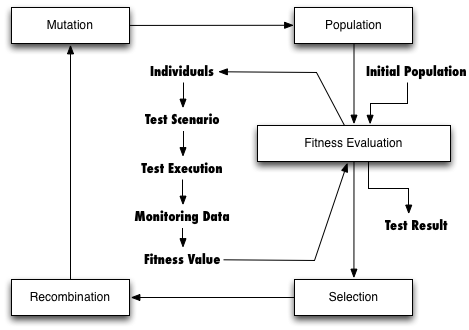
\includegraphics[width=1\textwidth]{./images/evolutionary.png}
\caption{Evolutionary Algorithm Search Based Test Cycle\cite{Baars2011}. }
\label{fig:evocycle}
\end{minipage}
\begin{minipage}{.5\textwidth}
\centering
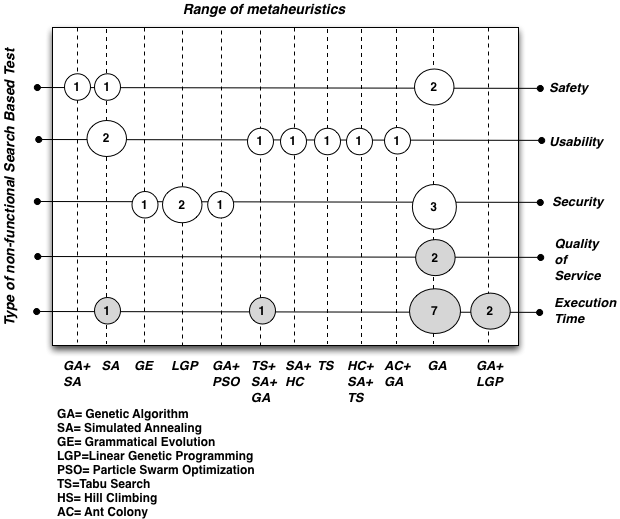
\includegraphics[width=1\textwidth]{./images/metaheuristics.png}
\caption{Range of metaheuristics by Type of non-functional Search Based Test\cite{Afzal2009a}. }
\label{fig:metabykind}
\end{minipage}
\end{figure}



First, a population of possible solutions to a problem
is created, usually at random. Starting with randomly
generated individuals results in a spread of solutions ranging in fitness because they are scattered around the search–space. Next, each individual in the population is evaluated by calculating its fitness via a fitness function. The principle idea of an Evolutionary Algorithm is that fit individuals survive over time and form even fitter individuals in future
generations. Selected individuals are then recombined
via a crossover operator. After crossover, the resulting offspring individuals may be subjected to a mutation operator. The algorithm iterates until a global optimum is reached or another stopping condition is fulfilled \cite{Baars2011}. 

The fitness evaluation is the most
time consuming task of SBST. However, for time consuming functional testing of complex industrial systems, minimizing
the number of generated individuals may also be highly desirable. This might be done using an assumption about
the "potential" of individuals in order to predict which individuals are likely to contribute to any future improvement.
This prediction could be achieved by using information about similar individuals that have been executed in earlier generations.



\subsection{Non-functional Search-Based Testing}

SBST has made many achievements, and demonstrated its wide applicability and increasing uptake. Nevertheless, there are pressing open problems and challenges that need more attention like to extend SBST to test non-functional properties, a topic that remains relatively under-explored, compared to structural testing. There are many kinds of non-functional search based tests  \cite{Afzal2009a}:

\begin{itemize}
\item Execution time: The application of evolutionary algorithms to find the best and worst case execution times (BCET, WCET).
\item Quality of service: uses metaheuristic search techniques to search violations of service level agreements (SLAs).
\item Security: apply a variety of metaheuristic search techniques  to detect security vulnerabilities like detecting buffer overflows.
\item Usability: concerned with construction of covering array which is a combinatorial object.
\item Safety: Safety testing is an important component of the testing strategy of safety critical systems where the systems are required to meet safety constraints.
\end{itemize}

A variety of metaheuristic search techniques are found to be applicable for non-functional testing including simulated annealing, tabu search, genetic algorithms, ant colony methods, grammatical evolution, genetic programming and swarm intelligence methods. The Fig. \ref{fig:metabykind} shows a comparison between the range of metaheuristcs and the type of non-functional search based test.The Data comes from Afzal et al. \cite{Afzal2009a}. Afzal's work adds to some of the latest research in this area (\cite{Garousi2006} \cite{Garousi2010} \cite{DiAlesio2013} \cite{DiAlesio2014} \cite{Alesio2015} \cite{Gois2016}). 





\section{Search-Based Stress Testing}

The search for the longest execution time is regarded as a discontinuous, nonlinear, optimization problem, with the input domain of the system under test as a search space \cite{Sullivan}.  The application of SBST algorithms to  stress tests involves finding the best- and worst-case execution times (B/WCET) to determine whether timing constraints are fulfilled \cite{Afzal2009a}. 

There are two measurement units normally associated with the fitness function in stress test: processor cycles and execution time. The processor cycle approach describes a fitness function in terms of processor cycles. The execution time approach involves executing the application under test and measuring the execution time \cite{Afzal2009a} \cite{tracey2000search}.

Processor cycles measurement is deterministic in the sense that it is independent of system load and results in the same execution times for the same set of input parameters. However, such a measurement is dependent on the compiler and optimizer used, therefore, the processor cycles differ for each platform. Execution time measurement is a non deterministic approach, there is no guarantee to get the same results for the same test inputs \cite{Afzal2009a}.  However, stress testing where testers have no access to the production environment should be measured by the execution time measurement \cite{Molyneaux2009} \cite{Afzal2009a}.

Table \ref{tab:comparison}  shows a comparison between the research studies on load, performance, and stress tests presented by Afzal et al. \cite{Afzal2009a}. Afzal's work adds to some of the latest research in this area (\cite{Garousi2006} \cite{Garousi2010} \cite{DiAlesio2013} \cite{DiAlesio2014} \cite{Alesio2015} \cite{Gois2016} ). The columns represent the type of tool used (prototype or functional tool), and the rows represent the metaheuristic approach used by each research study (genetic algorithm, Tabu search, simulated annealing, or a customized algorithm). The table also sorts the research studies by the type of fitness function used (execution time or processor cycles). 


\begin{table}[h]
\centering
\caption{Distribution of the research studies over the range of applied metaheuristics}
\label{tab:comparison}
\begin{tabular}{p{2.2cm}|p{2.8cm}|p{2.8cm}|p{2.8cm}|}
\cline{2-4}
                                                                & \multicolumn{2}{c|}{\textbf{Prototypes}}            & \textbf{Functional Tool} \\ \cline{2-4} 
                                                                & \begin{minipage}{0.2\textwidth}\footnotesize Execution Time  \end{minipage}          & \begin{minipage}{0.2\textwidth}\footnotesize Processor Cycles \end{minipage}        & \begin{minipage}{0.2\textwidth}\footnotesize Execution Time \end{minipage}           \\ \cline{2-4} 
%\setlength{\extrarowheight}{20pt}
\begin{tabular}[c]{@{}l@{}}\begin{minipage}{0.1\textwidth}\scriptsize GA + SA  \\ + Tabu \\ Search \end{minipage}\end{tabular}  & \cellcolor[HTML]{FFFFFF} & \cellcolor[HTML]{FFFFFF} & \cellcolor[HTML]{FFFFFF} \begin{minipage}{0.2\textwidth} \tiny Gois et al. 2016 \cite{Gois2016}  \end{minipage}  \\[2ex] \cline{2-4} 
\begin{minipage}{0.1\textwidth}\scriptsize GA \end{minipage}                                                              & \cellcolor[HTML]{FFFFFF} \begin{minipage}{0.12\textwidth}   \tiny \textnormal{ \\  Alander et al.,1998 \cite{Alander} \\ Wegener et al., 1996 and 1997 \cite{Wegener1997}\cite{J.WegenerK.GrimmM.GrochtmannH.Sthamer1996} \\  Sullivan et al., 1998 \cite{Sullivan} \\ Briand et al., 2005 \cite{Briand2005} \\ Canfora et al., 2005 \cite{Canfora}  \\ }\end{minipage} & \cellcolor[HTML]{FFFFFF} \begin{minipage}{0.12\textwidth} \tiny \textrm{  \\ Wegener and Grochtmann, 1998 \cite{Wegener1998} \\  Mueller et al., 1998 \cite{Mueller1998} \\ Puschner et al. \cite{Puschner1998} \\ Wegener et al., 2000 \cite{Stations} \\ Gro et al., 2000 \cite{Gross2000}  \\ }\end{minipage}& \cellcolor[HTML]{FFFFFF} \begin{minipage}{0.12\textwidth}   \tiny \textnormal{ \\  Di Penta, 2007 \cite{Penta2007} \\ Garoussi, 2006 \cite{Garousi2006} \\ Garousi, 2008 \cite{Garousi2008} \\ Garousi, 2010 \cite{Garousi2010} \\ } \end{minipage} \\[2ex] \cline{2-4} 
\begin{minipage}{0.1\textwidth}\scriptsize Simulated \\ Annealing \\ (SA) \end{minipage}                                                             & \cellcolor[HTML]{FFFFFF} & \cellcolor[HTML]{FFFFFF} & \cellcolor[HTML]{FFFFFF} \begin{minipage}{0.12\textwidth}   \tiny  Tracey, 1998 \cite{Tracey1998} \end{minipage} \\[2ex] \cline{2-4}
\begin{minipage}{0.1\textwidth}\scriptsize  Constraint \\ Programming \end{minipage}                                                             & \cellcolor[HTML]{FFFFFF} & \cellcolor[HTML]{FFFFFF} & \cellcolor[HTML]{FFFFFF} \begin{minipage}{0.12\textwidth}   \tiny  Alesio, 2014 \cite{DiAlesio2014} \\ Alesio, 2013 \cite{DiAlesio2013}  \end{minipage} \\[2ex] \cline{2-4} 
\begin{minipage}{0.1\textwidth}\scriptsize  GA +\\ Constraint \\ Programming \end{minipage}                                                             & \cellcolor[HTML]{FFFFFF} & \cellcolor[HTML]{FFFFFF} & \cellcolor[HTML]{FFFFFF} \begin{minipage}{0.12\textwidth}   \tiny  Alesio, 2015 \cite{Alesio2015} \end{minipage} \\[2ex] \cline{2-4} 
\setlength{\extrarowheight}{20pt}
\begin{tabular}[c]{@{}l@{}}
\begin{minipage}{0.1\textwidth}\scriptsize Customized \\ Algorithm \end{minipage}\end{tabular} & \cellcolor[HTML]{FFFFFF} & \cellcolor[HTML]{FFFFFF}  \begin{minipage}{0.12\textwidth}   \tiny  \textnormal{   \raggedleft Pohlheim, 1999 \cite{Pohlheim2005}  } \end{minipage} & \cellcolor[HTML]{FFFFFF} \\[4ex] \cline{2-4}
\end{tabular}
\end{table}

The studies can be grouped into two main groups:

\begin{itemize}
\item Search-Based Stress Tesing on Safety-critical systems.
\item Search-Based Stress Testing on Industrial systems.
\end{itemize}


\subsection{Search-Based Stress Tesing on Safety-critical systems}

Domains such as avionics, automotive and aerospace feature safety-critical systems, whose failure could result in catastrophic consequences.  The importance
of software in such systems is permanently increasing due to the need of a higher system
flexibility. For this reason, software components of these systems are usually subject to safety certification. In this context, software safety certification has to take into account performance requirements specifying constraints on how the system should react to its environment, and how it should execute on its hardware platform \cite{DiAlesio2013}.

Usually, embedded computer systems have to fulfil real-time requirements. A faultless function of the systems does not depend only on their logical correctness but also on their temporal correctness. Dynamic aspects like the duration of computations, the memory actually needed during program execution, orthe synchronisation of parallel processes are of major importance for the correct function of real-time systems  \cite{J.WegenerK.GrimmM.GrochtmannH.Sthamer1996} .

The concurrent nature of embedded software makes  the order of external events triggering the systems tasks is often unpredictable. Such increasing software complexity
renders performance analysis and testing increasingly
challenging. This aspect is reflected by the fact that most existing testing approaches target system functionality rather than performance \cite{DiAlesio2013}.

Reactive real-time systems must react to external events within time constraints. Triggered tasks must execute within deadlines. Shousha develops a methodology for the derivation of test cases that aims at maximizing the chance of critical deadline misses \cite{shousha2003performance}. 

The main goal of Search-Based Stress testing of Safety-critical systems it is finding a combination of inputs that causes the system to delay task completion to the greast extent possible \cite{shousha2003performance}. The followed approaches uses metaheuristics to discover the worst-case execution times. 

Wegener et al. \cite{Wegener1997} used genetic algorithms(GA) to search for input situations that produce very long or very short execution times. The fitness function used was the execution time of an individual measured in micro seconds \cite{Wegener1997}. Alander et al. \cite{Alander} performed experiments in a simulator environment to measure response time extremes of protection relay software using genetic algorithms. The fitness function used was the response time of the tested software. The results showed that GA generated more input cases with longer response times \cite{Alander}. 

Wegener and Grochtmann performed a  experimentation
to compare GA with random testing. The fitness function used was duration of execution measured in processor cycles.  The results showed that, with a large number of input parameters, GA obtained more extreme execution times with less or equal testing effort than random testing \cite{J.WegenerK.GrimmM.GrochtmannH.Sthamer1996} \cite{Wegener1998}.


Gro et. al. \cite{Gross2000} presented a prediction model  which can be used to predict evolutionary testability. The research confirmed that there is a relationship between the complexity of a test object and the ability of a search algorithm to produce input parameters according to B/WCET \cite{Gross2000}. 

Briand et al. \cite{Briand2005} used GA to find the sequence of arrival times of events for aperiodic tasks, which will cause the greatest delays in the execution of the target task. A prototype tool named real-time test tool (RTTT) was developed to facilitate the execution of runs of genetic algorithm. Two case studies were conducted and results illustrated that RTTT was a useful tool to stress a system under test \cite{Briand2005}.


Pohlheim and Wegener used an extension of genetic algorithms with multiple sub-populations, each using a different search strategy. The duration of execution measured in processor cycles was taken as the fitness
function. The GA found longer execution times for all the given modules in comparison with systematic testing\cite{Pohlheim2005}.

Garousi presented a stress test methodology aimed at increasing chances of discovering faults related to distributed traffic in distributed systems. The technique uses as input a specified UML 2.0 model of a system, augmented with timing information.The results indicate that the technique is significantly more effective at detecting distributed traffic-related faults when compared to standard test cases based on an operational profile \cite{Garousi2006}.

Alesio, Nejati and Briand describe a approach based
on Constraint Programming (CP) to automate the generation of test cases that reveal, or are likely to, task deadline misses. They evaluate it through a comparison with a state-of-the-art approach based on Genetic Algorithms (GA). In particular, wthe study compares CP and GA in five case studies for efficiency, effectiveness, and scalability. The experimental results show that, on the largest and more complex case studies, CP performs significantly better than GA. The research proposes a tool-supported, efficient and effective approach based on CP to generate stress test cases that maximize the likelihood of task deadline misses \cite{DiAlesio2013}.

Alesio describe stress test case generation as a search problem over the space of task arrival times. The research search for worst case scenarios maximizing deadline misses where each scenario characterizes a test case. The paper combine two strategies, GA and Constraint Programming (CP). The results show that, in comparison with GA and CP in isolation, GA+CP achieves nearly the same effectiveness as CP and the same efficiency and solution diversity as GA, thus combining the advantages of the two strategies. Alesio concludes that a combined GA+CP approach to stress testing is more likely to scale to large and complex systems \cite{Alesio2015}.

\subsection{Search-Based Stress Testing on Industrial systems} 

Usually, the application of Search-Based Stress Testing on non safety-critical systems deals with the generation of test cases that causes Service Level Agreements violations.


Tracey et al. \cite{Tracey1998} used simulated annealing (SA) to test four
simple programs. The results of the research presented that the use of SA was more effective with larger parameter space. The authors highlighted the need of a detailed comparison of various optimization techniques to explore WCET and BCET of the of the system under test \cite{Tracey1998}.

Di Penta et al. \cite{Penta2007} used GA to create test data that violated QoS constraints causing SLA violations. The generated test data included combinations of inputs. The approach was applied to two case studies. The first case study was an audio processing workflow. The second case study, a service producing charts, applied the black-box approach with fitness calculated only on the basis of how close solutions violate QoS constraint. The genome representation is presented in Fig \ref{fig:dipenta}. The representation models a wsdl request to a webservice.

\begin{figure}[h]
\centering
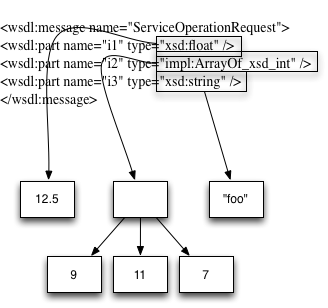
\includegraphics[width=0.6\textwidth]{./images/dipenta.png}
\caption{Genome representation \cite{Penta2007}. }
\label{fig:dipenta}
\end{figure}



In case of audio workflow, the GA outperformed random search. For the second case study, use of black-box approach successfully violated the response time constraint, showing the violation of QoS constraints for a real service available on the Internet \cite{Penta2007}.


Gois et al. proposes an hybrid metaheuristic approach using genetic algorithms, simulated annealing, and tabu search algorithms to perform stress testing. A tool named IAdapter, a JMeter plugin used for performing search-based stress tests, was developed. Two experiments were performed to validate the solution. In the first experiment, the signed-rank Wilcoxon non- parametrical procedure was used for comparing the results. The significant level adopted was 0.05. The procedure showed that there was a significant improvement in the results with the Hybrid Metaheuristic approach.
In the second experiment, the whole process of stress and performance tests, which took 3 days and about 1800 executions, was carried out without the need for monitoring by a test designer. The tool automatically selected the next scenarios to be run up to the limit of six generations previously established \cite{Gois2016}. 

\section{Metaheuristics and Hybrid Metaheuristics}

In the computer science, the term metaheuristic is accepted for general techniques which are not specific to a particular problem. A metaheuristic is formally defined as an iterative generation process which guides a subordinate heuristic by combining intelligently different concepts for exploring and exploiting the search space \cite{raidl2010metaheuristic}. 

Metaheuristics are strategies that guide the search process to efficiently explore the search space in order to find optimal solutions. Metaheuristic algorithms are approximate and usually non-deterministic and sometimes incorporate mechanisms to avoid getting trapped in confined areas of the search space. There are different ways to classify and describe metaheuristic algorithm \cite{Blum2003}:

\begin{itemize}
\item Nature-inspired vs. non-nature inspired. There are nature-inspired algorithms, like Genetic Algorithms and Ant Algorithms, and non nature-inspired ones such as Tabu Search and Iterated Local Search. 

\item Population-based vs. single point search. Algorithms working on single solutions are called trajectory methods, like Tabu Search, Iterated Local Search and Variable Neighborhood Search. They all share the property of describing a trajectory in the search space during the search process. Population-based metaheuristics perform search processes which describe the evolution of a set of points in the search space.

\item One vs. various neighborhood structures. Most metaheuristic algorithms work on one single neighborhood structure. In other words, the fitness landscape topology does not change in the course of the algorithm. Other metaheuristics, such as Variable Neighborhood Search (VNS), use a set of neighborhood structures which gives the possibility to diversify the search by swapping between different fitness
landscapes.
\end{itemize}

\subsection{Single-Solution Based Metaheuristics}

While solving optimization problems, single-solution based metaheuristics improve a single solution. They could be viewed as "walks" through neighborhoods or search trajectories through the search space of the problem at hand.
 

\subsubsection{Neighborhood}

The definition of Neighborhood is a required common step for the design of any Single-Solution metaheuristic (S-metaheuristic). The neighborhood structure it is a important piece in the performance of an S-metaheuristic. If the neighborhood structure is not adequate to the problem,
any S-metaheuristic will fail to solve the problem. The neighborhood function N is a mapping: $ N : S \rightarrow N\textsuperscript{2} $ that assigns to each solution s of \textit{S} a set of solutions \textit{N(s)}$\subset$ S \cite{Talbi2013}.

The neighborhood definition depends  representation associated with the problem. For permutation-based representations, a usual neighborhood is based on the swap operator that consists in swapping the location of two elements $s_i$ and $s_j$ of the permutation \cite{Talbi2013}. The Fig. \ref{fig:sperneighborhood} presents a example where a set of neighbors is found by permutation. 


\begin{figure}[h]
\centering
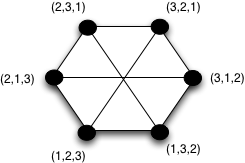
\includegraphics[width=0.6\textwidth]{./images/neighborhood.png}
\caption{ An example of neighborhood for a permutation \cite{Talbi2013}.}
\label{fig:sperneighborhood}
\end{figure}



Single-Solution Based Metaheuristics methods are characterized by a trajectory in the search space. Two common S-metaheuristics methods are Simulated Annealing and Tabu Search.


\subsubsection{Simulated Annealing}

Simulated Annealing (SA) is a randomized algorithm that tries to avoid being trapped in local optimum solution by assigning probabilities to deteriorating moves. The SA procedure is inspired from the annealing process of solids. SA is based on a physical
process in metallurgy discipline or solid matter physics. Annealing is the process of obtaining low energy states of a solid in heat treatment \cite{Jaziri2008}. 

The algorithmic framework of SA is described in Alg. \ref{sa}.  The algorithm starts by generating an initial solution in function \textit{GenerateInitialSolution()}. The initial temperature value is determined in function \textit{SetInitialTemperature()} such that the probability for an uphill move is quite high at the start of the algorithm. At each iteration a solution $\mbox{s}_1$ is randomly chosen in function \textit{PickNeighborAtRandom(N(s))}. If \textit{$\mbox{s}_1$} is better than \textit{s}, then \textit{$\mbox{s}_1$} is accepted as new current solution. Else, if the move from \textit{s} to \textit{$\mbox{s}_1$} is an uphill move, \textit{$\mbox{s}_1$}  is accepted with a probability which is a function of a temperature parameter \textit{Tk} and \textit{s} \cite{raidl2010metaheuristic}. 

\begin{algorithm}[h]
  \caption{Simulated Annealing Algorithm}\label{sa}
  \begin{algorithmic}[1]
    
    \State $s\gets GenerateInitialSolution()$
    \State $k\gets 0 $
    \State $Tk\gets SetInitialTemperature()$
    \While{termination conditions not met }
    \State $\mbox{s}_1\gets PickNeighborAtRandom(N (s))$
    \If{$(f(\mbox{s}_1)<f(s))$}
    \State $s\gets\mbox{s}_1$
    \Else $\;$ Accept $\mbox{s}_1$ as new solution with probability p($\mbox{s}_1|$Tk,s) 
    \EndIf
    \State $K\gets K+1$
    \State $Tk\gets AdaptTemperature()$
    \EndWhile
      
  \end{algorithmic}
\end{algorithm}

\subsubsection{Tabu Search}

Tabu Search (TS) is a metaheuristic that guides a local heuristic search procedure to explore the solution space beyond local optimal and search with short term memory to avoid cycles. Tabu Search uses a  tabu list to keep track of the last  moves, and don’t allow going back to these \cite{Glover1986}.

The basic idea of TS is the explicit use of search history, both to escape
from local minima and to implement a strategy for exploring the search space.
A basic TS algorithm uses short term memory in the form of socalled
tabu lists to escape from local minima and to avoid cycles \cite{Tobergte2013}.

The algorithmic framework of Tabu Search is described in Alg. \ref{tsa}.  The algorithm starts by generating an initial solution in function \textit{GenerateInitialSolution()} and the tabu lists are initialized as empty lists in function \textit{InitializeTabuLists($\mbox{TL}_1$,...,$\mbox{TL}_r$)}. For performing a move, the algorithm first determines those solutions from the neighborhood \textit{N(s)} of the current solution \textit{s} that contain solution features currently to be found in the tabu lists. They are excluded from the neighborhood, resulting in a restricted set of neighbors \textit{$\mbox{N}_a(s)$}. At each iteration the best solution \textit{$\mbox{s}_1$} from \textit{$\mbox{N}_a(s)$} is chosen as the new current solution. Furthermore, in procedure \textit{UpdateTabuLists($\mbox{TL}_1$,...,$\mbox{TL}_r$,s,$\mbox{s}_1$)} the corresponding features of this solution are added to the tabu lists.


\begin{algorithm}[h]
  \caption{Tabu Search Algorithm}\label{tsa}
  \begin{algorithmic}[2]
    
    \State $s\gets GenerateInitialSolution()$
    \State InitializeTabuLists($\mbox{TL}_1$,...,$\mbox{TL}_r$)
    \While{termination conditions not met }
    \State $\mbox{N}_a(s)\gets$ $\{\mbox{s}_1 \in N(s) |\mbox{s}_1$ does not violate a tabu condition, or it satisfies at least one aspiration condition $\}$ 
    \State $\mbox{s}_1\gets argmin\{f(\mbox{s}_2)|\mbox{s}_2 \in \mbox{N}_a(s) \}$
    \State UpdateTabuLists($\mbox{TL}_1$,...,$\mbox{TL}_r$,s,$\mbox{s}_1$)
    \State $s\gets \mbox{s}_1$
    \EndWhile
      
  \end{algorithmic}
\end{algorithm}

\subsection{Population-based metaheuristics}

Population-based metaheuristics (P-metaheuristics) could be viewed as an iterative improvement in a population of solutions. First, the population is initialized. Then, a new population of solutions is generated. Finally, this new population is integrated into the current one using some selection procedures. The search process is stopped when a stopping criterion is satisfied. Algorithms such as Genetic algorithms (GA), scatter search (SS), estimation of distribution algorithms (EDAs), particle swarm optimization (PSO), bee colony (BC), and artificial immune systems (AISs) belong to this class of metaheuristics \cite{talbi2009metaheuristics}. 

\subsection{Genetic Algorithms}

Genetic Algorithms could be a mean of solving complex optimization problems that are often NP Hard. GAs are based on concepts adopted from genetic and evolutionary theories. GAs are comprised of several components \cite{hong2000simultaneously} \cite{shousha2003performance} :

\begin{itemize}
\item a representation of the solution, refered as the chromossome;
\item fitness of each chromossome, refered as objective function;
\item the genetic operations of crossover and mutation which generate new offspring. 
\end{itemize}


Algorithm \ref{gna} shows the basic structure of GA algorithms. In this algorithm, P denotes the population of individuals. A population of offspring is generated by the application of recombination and mutation operators and the individuals for the next population are selected from the union of the old population and the offspring population \cite{raidl2010metaheuristic}.


\begin{algorithm}[h]
  \caption{Genetic Algorithm}\label{gna}
  \begin{algorithmic}[3]
    
    \State $s\gets GenerateInitialSolution()$
    \State Evaluate(P)
    \While{termination conditions not met }
    \State $\mbox{P}_1\gets$ $Recombine(P)$
    \State $\mbox{P}_2\gets$ $Mutate(\mbox{P}_1)$ 
    \State $Evaluate(\mbox{P}_2)$
    \State $P\gets Select(\mbox{P}_2,P)$
    \EndWhile
      
  \end{algorithmic}
\end{algorithm}

\subsection{Hybrid  Metaheuristics}

However, in recent years it has become evident that the concentration on a sole metaheuristic is rather restrictive. A skilled combination of a metaheuristic with other optimization techniques, a so called hybrid metaheuristic, can provide a more efficient behavior
and a higher flexibility when dealing with real-world and large-scale problems \cite{Talbi2012}.

A combination of one metaheuristic with components from other metaheuristics is called a hybrid metaheuristic. The concept of hybrid metaheuristics has been commonly accepted only in recent years, even if the idea of combining different metaheuristic strategies and algorithms dates back to the 1980s. Today, we can observe a generalized common agreement on the advantage of combining components from different search techniques and the tendency of designing hybrid techniques is widespread in the fields of operations research and artificial intelligence \cite{raidl2010metaheuristic}. 


There are two main categories of metaheuristic combinations: collaborative combinations and integrative combinations. These are presented in Fig. \ref{fig:metaheuristc} \cite{Raidl2006}.

\begin{figure}[h]
\begin{minipage}{.5\textwidth}
\centering
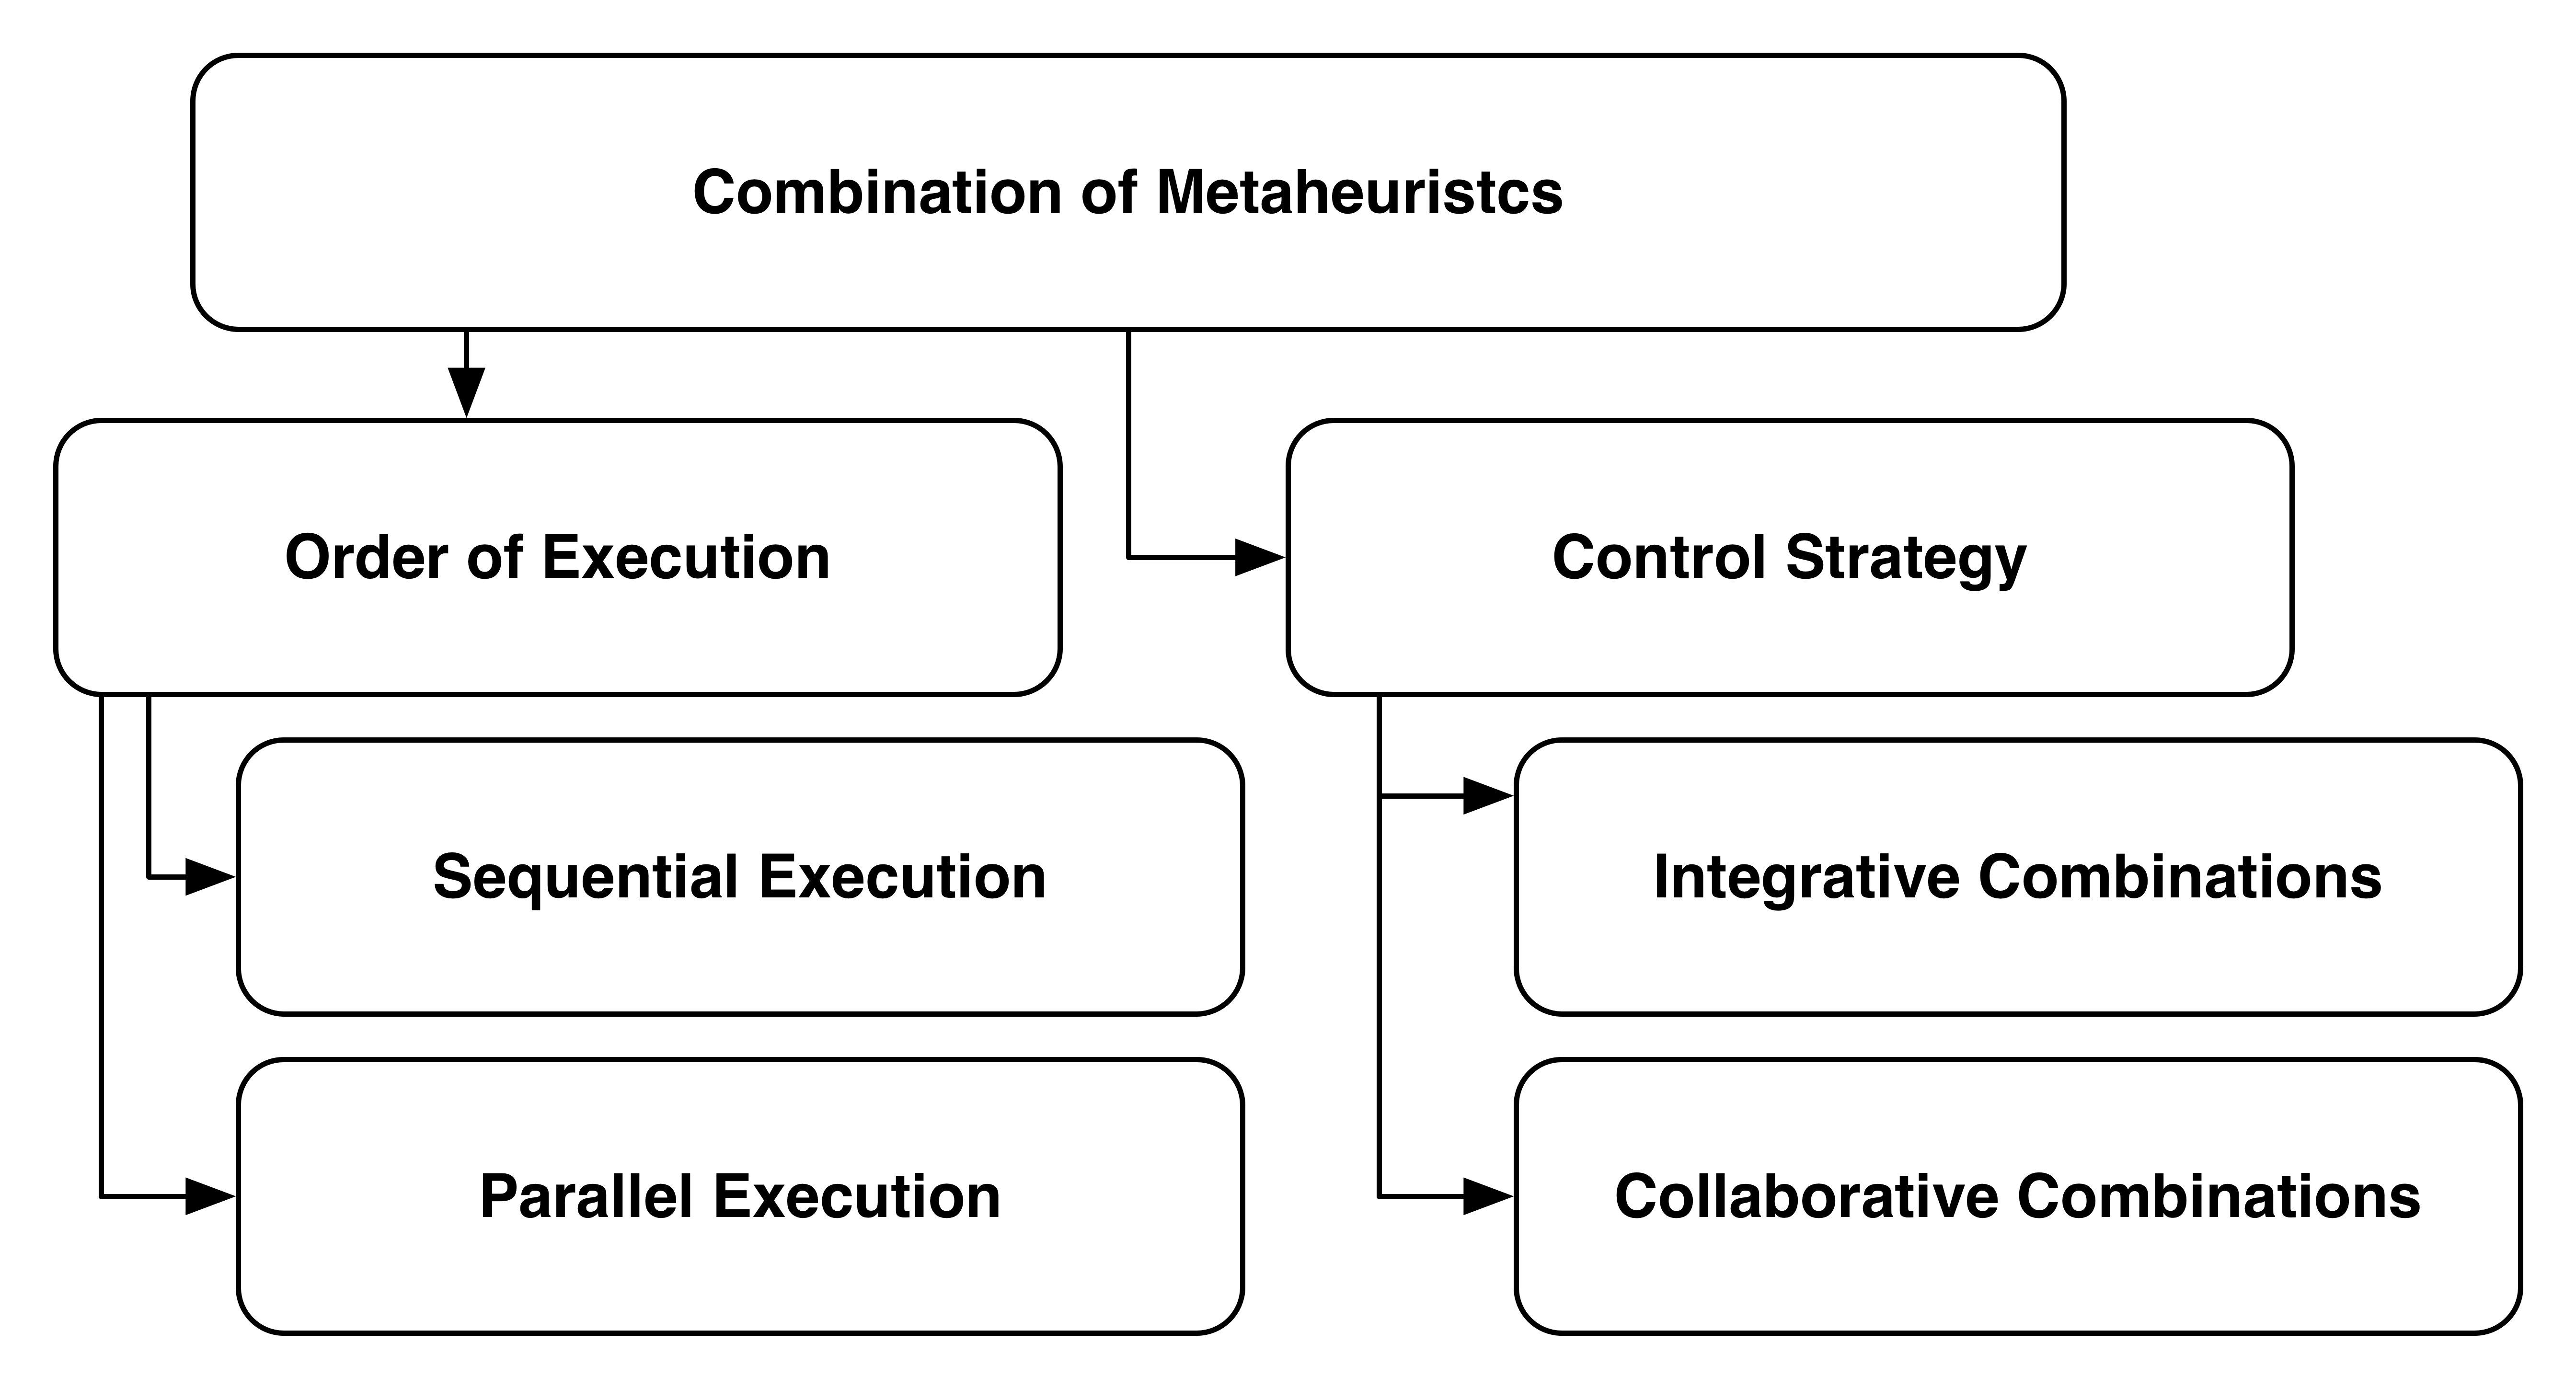
\includegraphics[width=1\textwidth]{./images/metaheuristc2.png}
\caption{Categories of metaheuristc combinations \cite{Puchinger2005} }
\label{fig:metaheuristc}
\end{minipage}
\begin{minipage}{.5\textwidth}
\centering
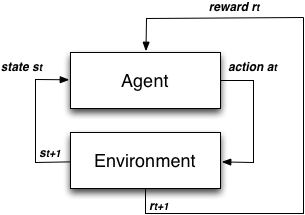
\includegraphics[width=1\textwidth]{./images/agentenv.png}
\caption{Example of interation between some agent and the environment}
\label{fig:agentenv}
\end{minipage}
\end{figure}

Collaborative combinations use an approach where the algorithms exchange information, but are not part of each other. In this approach, algorithms may be executed sequentially or in parallel. 

One of the most popular ways of metaheuristic hybridization consists in the use of trajectory methods inside population-based methods. Population-based methods are better in identifying promising areas in the search space from which trajectory methods can quickly reach good local optima. Therefore, metaheuristic hybrids that can effectively combine the strengths of both population-based methods and trajectory methods are often very successful \cite{raidl2010metaheuristic}.


The work uses a type of collaborative combination with sequential execution with two trajectory methods (Tabu Search and Simulated Annealing) and Genetic Algorithms.





\section{Q-Learning}




\subsection{Reinforcement Learning}

Reinforcement learning (RL) refers to both a learning problem and a subfield of machine
learning. As a learning problem, it refers to learning to control a system so as to maximize
some numerical value which represents a long-term objective. A typical setting where
reinforcement learning operates is shown in Figure \ref{fig:agentenv}: A controller receives the controlled
system’s state and a reward associated with the last state transition. It then calculates an
action which is sent back to the system.





The basis idea of Reinforcement learning  is simply to capture the most important aspects of the real problem facing a learning agent interacting with its environment to achieve a goal \cite{Sutton2012}. Reinforcement learning is learning what to do—how to map situations to actions—so as to maximize a numerical reward signal. The learner need to discover which actions yield the most reward by trying them \cite{Sutton2012}.

In Reinforcement Learning, an agent wanders in an unknown environment and tries to maximize its long term return by performing actions and receiving rewards. The challenge is to understand how a current action will affect future rewards. A good way to model this task is with Markov Decision Processes (MDP), which have become the dominant approach in Reinforcement Learning. There are two types of learning problems:

\begin{itemize}
\item Iteractive learning;
\item Non-interactive learning.
\end{itemize}

In non-interactive learning, the natural goal is to find a good policy given a fixed number of observations. A common situation is when the sample is fixed. For example, the sample can be the result of some experimentation with some physical system that happened before learning started. 

In Interactive learning, learning happens while interacting with a real system in a closed-loop fashion. A reasonable goal then is to optimize online performance,
making the learning problem an instance of online learning. Online performance can be measured in different ways. A natural measure is to use the sum of rewards incurred during learning. 

Interactive learning is potentially easier since the learner has the additional option to influence the distribution of the sample. However, the goal of
learning is usually different in the two cases, making these problems incomparable in general.

In Reinforcement Learging, all agents act in two phases: Exploration vs Explotation. In Exploration phase, the agents tries discover better action selections to improve its knowledge. In Explotation phase, the agents tries to maximize its reward, based on what its already know.

One of the challenges that arise in reinforcement learning is the trade-off between exploration and exploitation. To obtain a lot of reward, a reinforcement learning
agent must prefer actions that it has tried in the past and found to be effective in producing reward.
But to discover such actions, it has to try actions that it has not selected before. The agent has to exploit what it already knows in order to obtain reward, but it also has to explore in order to make better action selections in the future.





\subsection{Markov decision processes}

Markov decision processes (MDPs) provide a mathematical framework for modeling decision making. A countable MDP is defined as a triplet $M=(\chi,A,P_{0})$ \cite{Szepesvari2010}. where $\chi$ is a set of states, A is a set of actions. The transition probability kernel $P_{0}$ assigns to each state-action pair $(x, a) \in \chi x A $


The six main elements of a MDP are:(1) state of the system, (2) actions, (3) transition probabilities, (4) transition rewards, (5) a policy, and (6) a performance metric \cite{Sutton2012}.

\begin{figure}
\begin{minipage}{.5\textwidth}
\centering
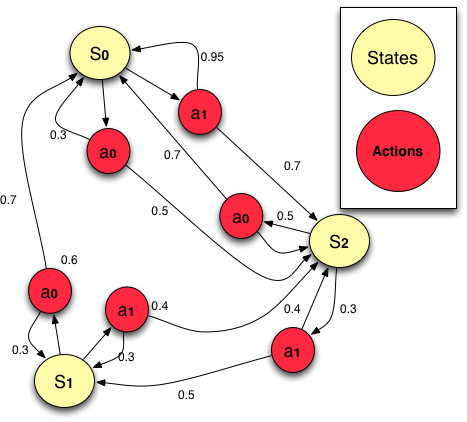
\includegraphics[width=1\textwidth]{./images/mdp1.png}
\caption{Example of a simple MDP with three states and two actions}
\label{fig:mdp}
\end{minipage}
\begin{minipage}{.5\textwidth}
\centering
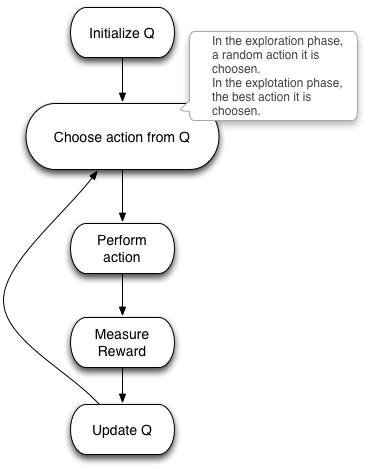
\includegraphics[width=0.8\textwidth]{./images/qalgo.png}
\caption{Q Learning algorithm}
\label{fig:qalgo}
\end{minipage}
\end{figure}



The state of a system is a parameter or a set of parameters that can be used to describe a system. For example the geographical coordinates of a robot can be used to
describe its state. A system whose state changes with time is called a dynamic system. Then it is not hard to see why a moving robot produces a dynamic system.

Actions are the controls allowed for an agent. Transition Probability denotes the probability of going from state i to state j under the influence of action a in one step. If an MDP has 3 states and 2 actions, there are 9 transition probabilities per action. Usually, the system receives an immediate reward ,which could be positive or negative, when it transitions from one state to another

A policy defines the learning agent’s way of behaving at a given time. Roughly speaking, a policy is a mapping from perceived states of the environment
to actions to be taken when in those states. It corresponds to what in
psychology would be called a set of stimulus–response rules or associations.  Policys mapping from states to actions.

Performance Metric: Associated with any given policy, there exists a so-called performance
metric — with which the performance of the policy is judged. Our goal is to select the policy
that has the best performance metric. 


\subsection{Q-Learning}

Q-learning is a model-free reinforcement learning technique. Q-learning, it is a multiagent learning algorithm that learns equilibrium policies in Markov games, just as Q-learning learns to optimal policies in Markov decision processes \cite{Greenwald2003}. 

Q-learning and related algorithms tries to learn the optimal policy from its history of interaction with the environment. A history of an agent is a sequence of state-action-rewards.Where $s_{n}$ it is a state, $a_{n}$ it is an action and $r_{n}$ is a reward:

\begin{equation}
<s_{0},a_{0},r_{1},s_{1},a_{1},r_{2},s_{2},a_{2},r_{3},s_{3},a_{3},r_{4},s_{4}....>,
\end{equation}


In Q-Learning, the system's objective is to learn a control policy $\pi = \sum_{n=0}^{\infty} \gamma\textsuperscript{n}  r_{t}+n $, where $\pi$  is the discounted cumulative reward, $\gamma$ is the discount rate ($01$) and $r_{t}$ is the reward reiceved after execution an action at time t. The fig. \ref{fig:qalgo} shows the summary version of Q-Learning algorithm. The first step it is to generate the initial state of the MDP. The second step it is to choose the best action or a random action based on the reward, the actions with best rewards are chosen.


\section{Improving Stress Search Based Testing using Q-Learning and Hybrid Metaheuristic Approach}


\subsection{Hybrid Approach}

A large number of researchers have recognized the advantages and huge potential of building hybrid metaheuristics. The main motivation for creating hybrid metaheuristics is to exploit the complementary character of different optimization strategies. In fact, choosing an adequate combination of algorithms can be the key to achieving top performance in solving many hard optimization problems \cite{Puchinger2005} \cite{Blum2012}.

The solution proposed by Gois et al. \cite{Gois2016} makes it possible to create a model that evolves during the test. The proposed solution model uses genetic algorithms, tabu search, and simulated annealing in two different approaches. The study initially investigated the use of these three algorithms. Subsequently, the study will focus in others Population-based and single point search metaheuristics. The first approach uses the three algorithms independently, and the second approach uses the three algorithms collaboratively (hybrid metaheuristic approach).

In the first approach , the algorithms do not share their best individuals among themselves. Each algorithm evolves in a separate way (Fig. \ref{fig:firstaproach}).





The second approach uses the algorithms in a collaborative mode (hybrid metaheuristic). In this approach, the three algorithms share their best individuals found (Fig. \ref{fig:secondapproach}). The next subsections present details about the used metaheuristic algorithms (Representation, initial population and fitness function).


\begin{figure}[h]
\begin{minipage}{.5\textwidth}
\centering
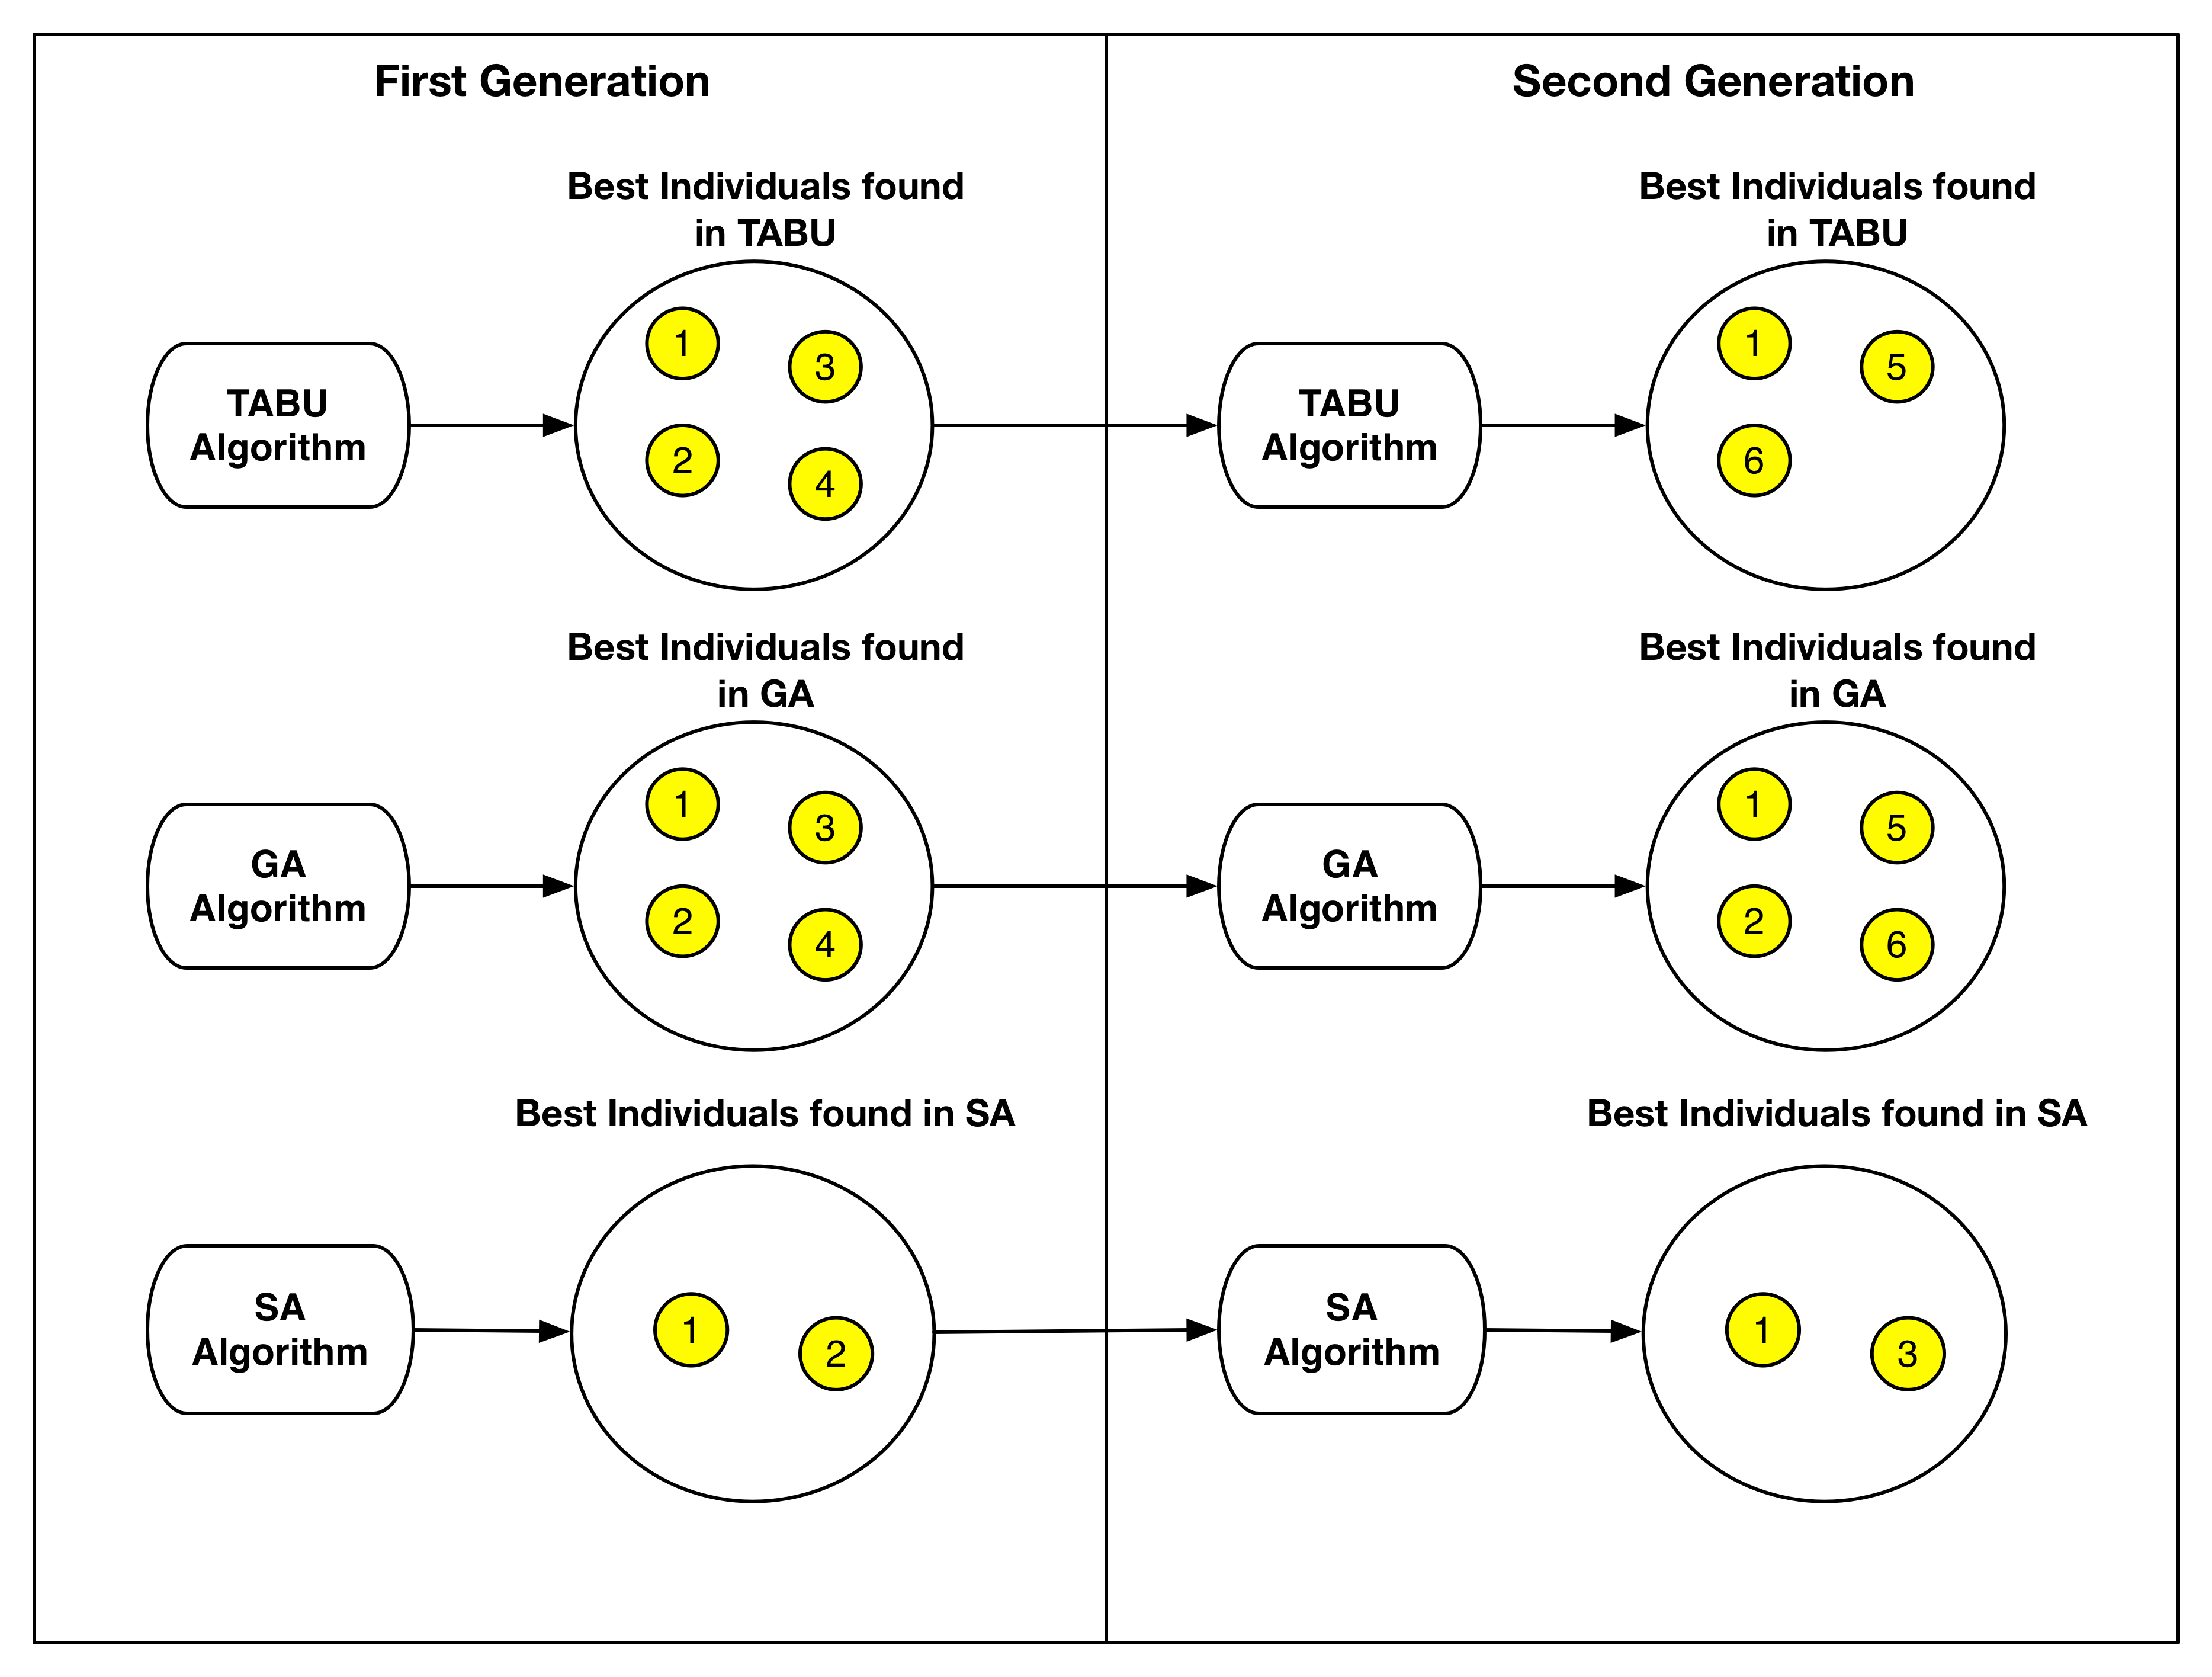
\includegraphics[width=1\textwidth]{./images/independ.png}
\caption{Use of the algorithms independently \cite{Gois2016}}
\label{fig:firstaproach}
\end{minipage}
\begin{minipage}{.5\textwidth}
\centering
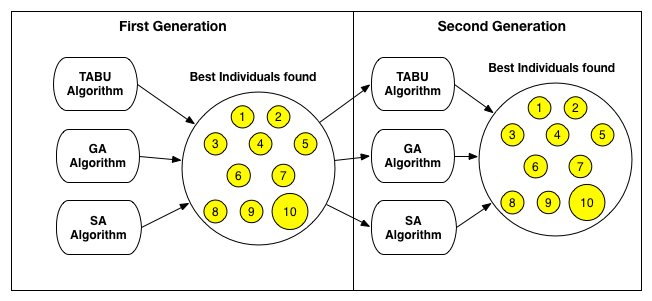
\includegraphics[width=1\textwidth]{./images/collaborative.png}
\caption{Use of the  algorithms collaboratively \cite{Gois2016}}
\label{fig:secondapproach}
\end{minipage}
\end{figure}

\subsubsection{Representation}

The solution representation is composed by a linear vector with 23 positions. The first position represents the name of an individual. The second position represents the algorithm (genetic algorithm, simulated annealing, or Tabu search) used by the individual. The third position represents the type of test (load, stress, or performance). The next positions represent 10 scenarios and their numbers of users. Each scenario is an atomic operation: the scenario must log into the application, run the task goal, and undo any changes performed, returning the application to its original state.

Fig. \ref{fig:genomarepresentation} presents the solution representation and an example using the crossover operation. In the example, genotype 1 has the Login scenario with 2 users, the Form scenario with 0 users, and the Search scenario with 3 users. Genotype 2 has the Delete scenario with 10 users, the Search scenario with 0 users, and the Include scenario with 5 users. After the crossover operation, we obtain a genotype with the Login scenario with 2 users, the Search scenario with 0 users, and the Include scenario with 5 users.

\begin{figure}[h]
\begin{minipage}{.5\textwidth}
\centering
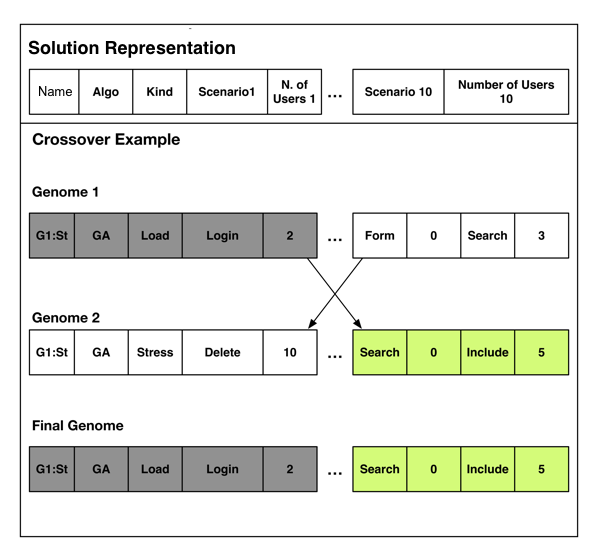
\includegraphics[width=1\textwidth]{./images/genomerepresentation1.png}
\caption{Solution representation and crossover example}
\label{fig:genomarepresentation}
\end{minipage}
\begin{minipage}{.5\textwidth}
\centering
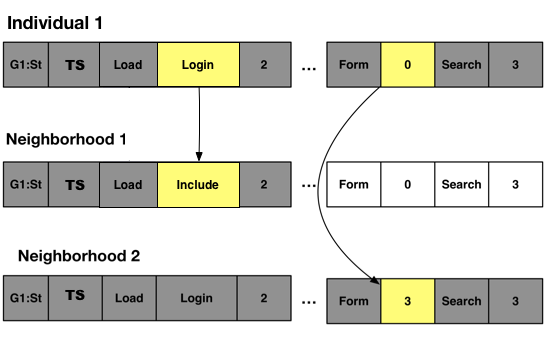
\includegraphics[width=1\textwidth]{./images/neighbor.png}
\caption{Tabu search and simulated annealing neighbor strategy}
\label{fig:neighbourtaby}
\end{minipage}
\end{figure}

Fig. \ref{fig:neighbourtaby} shows the strategy used by the proposed solution to obtain the representation of the neighbors for the Tabu search and simulated annealing algorithms. The neighbors are obtained by the modification of a single position (scenario or number of users) in the vector.





\subsubsection{Initial population}

The strategy used by the plugin to instantiate the initial population is to generate 50\% of the individuals randomly, and 50\% of the initial population is distributed in three ranges of values:

\begin{itemize}
\item Thirty percent of the maximum allowed users in the test;
\item Sixty percent of the maximum allowed users in the test; and
\item Ninety percent of the maximum allowed users in the test.
\end{itemize}

The percentages relates to the distribution of the users in the initial test scenarios of the solution. For example, in a hypothetical test with 100 users, the solution will create initial test scenarios with 30, 60 and 90 users.

\subsubsection{Objective (fitness) function}

The proposed solution was designed to be used with independent testing teams in various situations where the teams have no direct access to the environment where the application under test was installed. Therefore, the IAdapter plugin uses a measurement approach to the definition of the fitness function. The fitness function applied to the IAdapter solution is governed by the following equation:

\begin{equation}
\begin{aligned}
fit=90percentileweigth* 90percentiletime\\
+80percentileweigth*80percentiletime\\+
70percentileweigth*70percentiletime+\\
maxResponseWeigth*maxResponseTime+\\
numberOfUsersWeigth*numberOfUsers-penalty
\end{aligned}
\end{equation}

The proposed solution's fitness function uses a series of manually adjustable user-defined weights (90percentileweight, 80percentileweight,  70percentileweight, maxResponseWeight, and numberOfUsersWeight). These weights make it possible to customize the search plugin's functionality. A penalty is applied when an application under test takes a longer time to respond than the level of service. The penalty is calculated by the follow equation:

\begin{equation}
\begin{aligned}
penalty=100 * \Delta \\
\Delta=(t_{Current Response Time} - t_{Maximum Response Time Expected})\\
\end{aligned}
\end{equation}

\subsection{Hybrid Metaheuristic with Q-Learning Approach}

The HybridQ algorithm uses the GA, SA and Tabu Search algorithms in a collaborative approach in conjunction with Q-Learning technique. The biggest difference between the Hybrid and HybridQ algorithms is the application of a series of modifications on individuals based on the Q-Learning algorithm before each generation.

\begin{figure}[h!]
\center
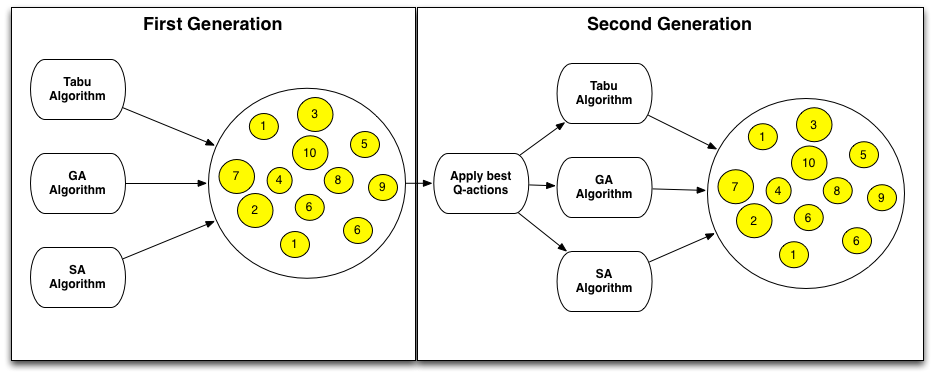
\includegraphics[width=1\textwidth]{./images/qhybrid.png}
\caption{Hybrid Metaheuristic with Q-Learning Approach}
\label{fig:hybridq}
\end{figure}

Figure \ref{fig:mdphybridq} shows the proposed MDP model for HybridQ. The model has three main states based on response time. A test may have a response time greater than 1.2 times the maximum response time alloowed, between 0.8 and 1.2 times the maximum response time allowed or less than 0.8 times the maximum response time allowed. A test receives a positive reward when an action increases fitnesse value and a negative reward when an action reduces the fitnesse value. The possible actions in MDP are the change of one of the test scenarios and increase or decrease of the number of users.

\begin{figure}[h!]
\begin{minipage}{.5\textwidth}
\center
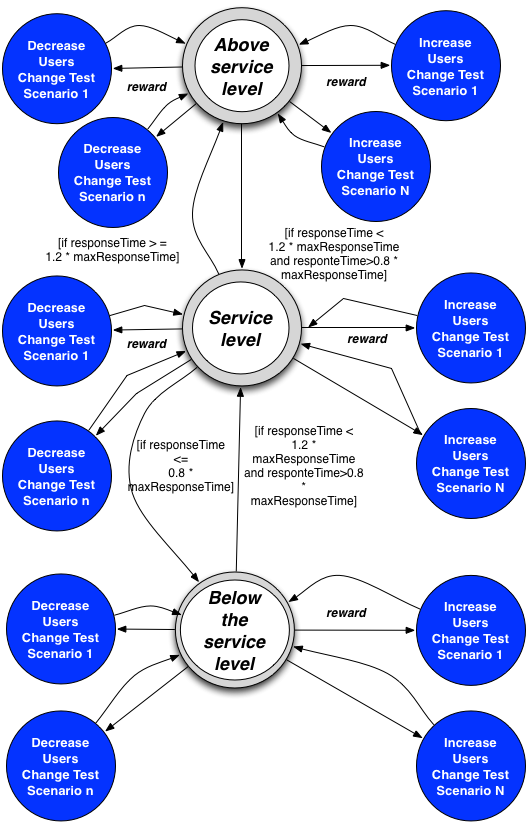
\includegraphics[width=1\textwidth]{./images/mdp3.png}
\caption{Markov Decision Process used by HybridQ}
\label{fig:mdphybridq}
\end{minipage}
\begin{minipage}{.5\textwidth}
\center
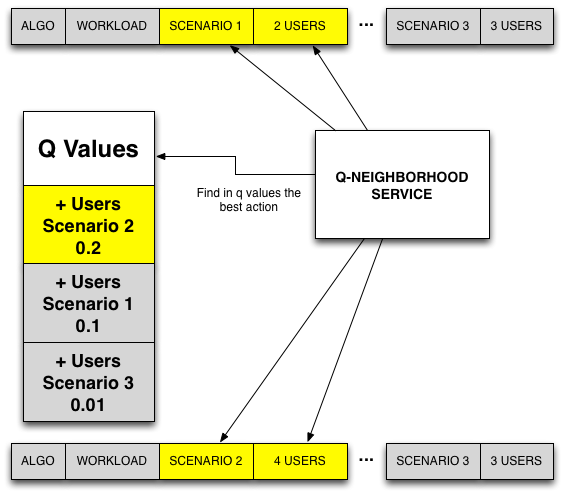
\includegraphics[width=1\textwidth]{./images/q-neighborservice.png}
\caption{HybridQ NeighborHood Service}
\label{fig:neighservice}
\end{minipage}
\end{figure}



Unlike the traditional approach, The update of Q values for each action also occurs in the explotation phase. The exploit phase ends when no value of Q it is equals zero for a state, ie, unlike the traditional approach an agent belonging to one state may be in the exploration phase while another agent may be in the explotation phase. The table presents an hyphotetical Q-values for a test. In the table \ref{pab:mdp}, it can be observed that the agents in the Service Level state are in the exploitation phase because there is no other value of Q equals to zero.


% Please add the following required packages to your document preamble:
% \usepackage[table,xcdraw]{xcolor}
% If you use beamer only pass "xcolor=table" option, i.e. \documentclass[xcolor=table]{beamer}
\begin{table}[]
\centering
\caption{Hypothetical MDP Q-values }
\label{pab:mdp}
\begin{tabular}{lll}
\rowcolor[HTML]{C0C0C0} 
\textbf{Above Service Level}  & \textbf{Scenario 1} & \textbf{Scenario 2} \\
Increment Users               & 0.2                 & 0.0                 \\
Reduce Users                  & 0.1                 & 0.2                 \\
Phase                         & Exploration         & Exploration         \\
\rowcolor[HTML]{C0C0C0} 
\textbf{Service Level}        & \textbf{Scenario 1} & \textbf{Scenario 2} \\
Increment Users               & 0.2                 & 0.11                \\
Reduce Users                  & 0.1                 & -0.2                \\
\rowcolor[HTML]{F8FF00} 
Phase                         & Explotation         & Explotation         \\
\rowcolor[HTML]{C0C0C0} 
\textbf{Bellow Service Level} & \textbf{Scenario 1} & \textbf{Scenario 2} \\
Increment Users               & 0.0                 & 0.2                 \\
Reduce Users                  & 0.1                 & 0.0                 \\
Phase                         & Exploration         & Exploration        
\end{tabular}
\end{table}

The Fig. \ref{fig:neighservice} presents how one of the neighbors of a test is generated using Q-Learning. The solution uses a service called Q-Neighborhood Service to generate the neighbor from the action that has the highest value of Q.




\subsection{IAdapter}

IAdapter is a JMeter plugin designed to perform search-based stress tests.  The plugin is available on www.iadapter.org.  The IAdapter plugin implements the solution proposed in Section 5. The next subsections present details about the Apache JMeter tool, the IAdapter Life Cycle and the IAdapter Components. The IAdapter plugin provides three main components: WorkLoadThreadGroup, WorkLoadSaver, and WorkLoadController. The Fig. \ref{fig:iadapterarchitecture} show the IAdapter architecture. All metaheuristic class implements the interface IAlgorithm. Test scenarios  and test results are stored in a Mysql database. GeneticAlgorithm class uses a framework named JGAP to implement Genetic Algorithms.

\begin{figure}[h]
\begin{minipage}{.5\textwidth}
\center
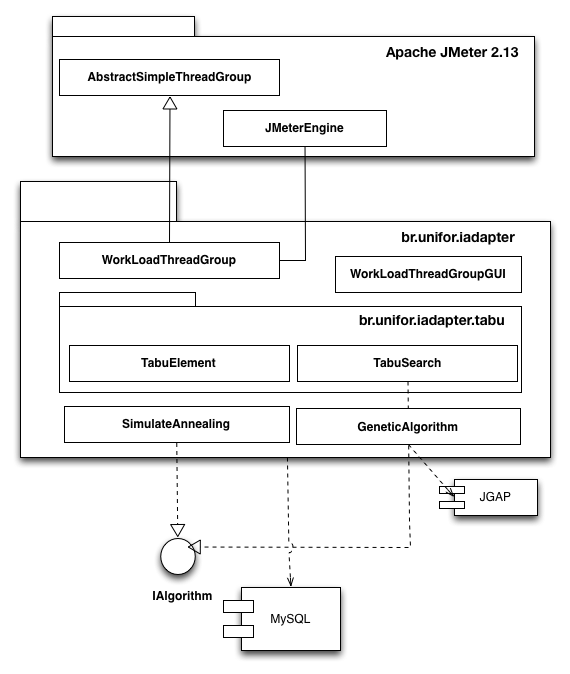
\includegraphics[width=1\textwidth]{./images/iadapter1.png}
\caption{IAdapter architecture}
\label{fig:iadapterarchitecture}
\end{minipage}
\begin{minipage}{.5\textwidth}
\centering
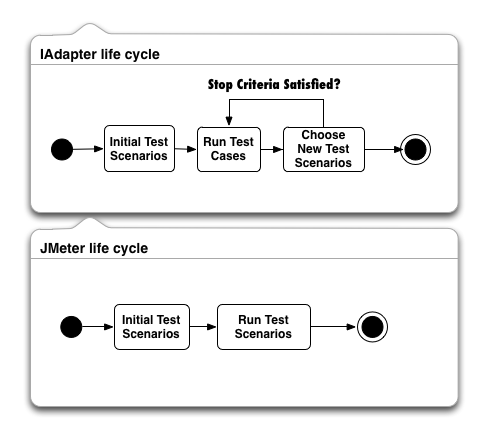
\includegraphics[width=1\textwidth]{./images/lifecycle2.png}
\caption{IAdapter life cycle}
\label{fig:iadapterlifecycle}
\end{minipage}
\end{figure}

The WorkLoadThreadGroup class is the Load Injection and Test Management modules, responsible to generate the initial population and uses the JMeter Engine to realize requests to server under test. 

\subsubsection{IAdapter Life Cycle}
 
Fig. \ref{fig:iadapterlifecycle} presents the IAdapter Life Cycle. The main difference between IAdapter and JMeter tool is that the IAdapter provide an automated test execution where the new test scenarios are choosen by the test tool.  In a test with JMeter, the tests scenarios are usually chosen by a test designer.



\subsubsection{IAdapter Components}
 
WorkLoadThreadGroup is a component that creates an initial population and configures the algorithms used in IAdapter. Fig. \ref{fig:tela1iadapter} presents the main screen of the WorkLoadThreadGroup component. The component has a name \ding{202}, a set of configuration tabs \ding{203}, a list of individuals by generation \ding{204}, a button to generate an initial population \ding{205}, and a button to export the results \ding{206}.

\begin{figure}[h]
\centering
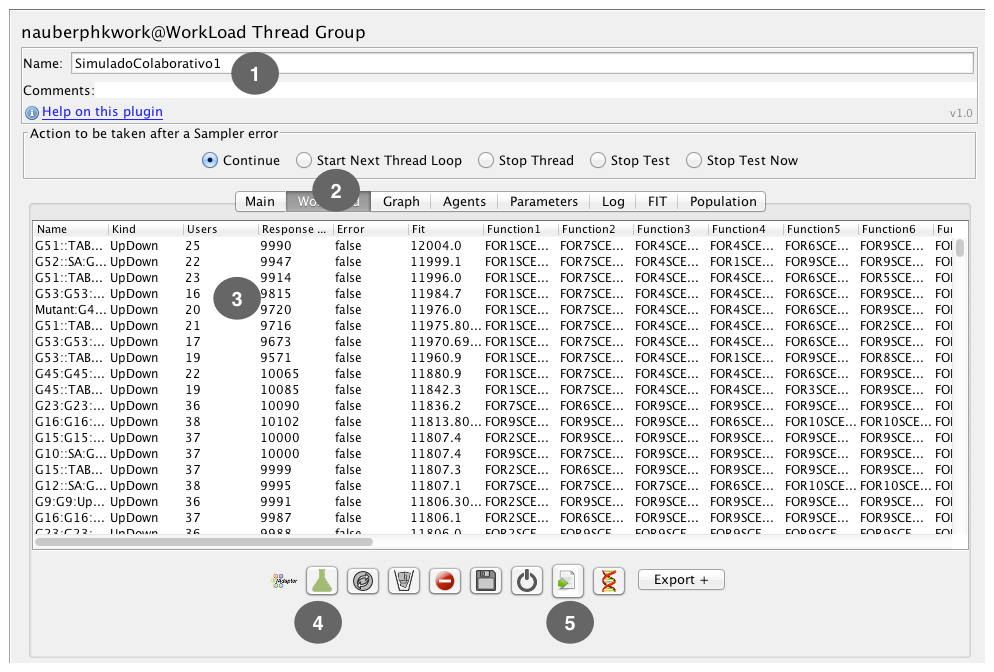
\includegraphics[width=0.8\textwidth]{./images/tela1iadapter.png}
\caption{WorkLoadThreadGroup component}
\label{fig:tela1iadapter}
\end{figure}

WorkLoadThreadGroup component uses the GeneticAlgorithm, TabuSearch and SimulateAnnealing classes.  The WorkLoadSaver component is responsible for saving all data in the database. The operation of the component only requires its inclusion in the test script.

WorkLoadController represents a scenario of the test. All actions necessary to test an application should be included in this component. All instances of the component need to login into the application under test and bring the application back to its original state.

\section{Experiments}

We conducted two experiments in order to verify the effectiveness of the HybridQ. The first experiment ran for 17 generations in an emulated evinronment. The experiments used an initial population of 4 individuals by metaheuristic. The genetic algorithm used the top 10 individuals from each generation in the crossover operation. The Tabu list was configured with the size of 10 individuals and expired every 2 generations.  The mutation operation was applied to 10\% of the population on each generation. The experiments uses tabu search, genetic algorithms and the hybrid metaheuristic approach proposed by Gois et al. \cite{Gois2016} and the HybridQ approach. 


The objective function applied is intended to maximize the number of users and minimize the response time of the scenarios being tested.  In this experiments, better fitness values meaning to find scenarios with more users and a low values of response time. A penalty is applied when the response time is greater than the  maximum response time expected. The experiments used the following fitness (goal) function. :

\begin{equation}
\begin{aligned}
fitness=3000*numberOfUsers\\
-20* 90percentiletime\\
-20*80percentiletime\\
-20*70percentiletime\\
-20*maxResponseTime\\
-penalty
\end{aligned}
\end{equation}

The experiments addresses:

\begin{itemize}
\item Validate the operation of the testbed tool.
\item Find the maximum number of users and the minimal response time.
\item Analyze and verify the best heuristics among those chosen to the experiments.
\end{itemize}


\begin{figure}[h]
\begin{minipage}{.5\textwidth}
\centering
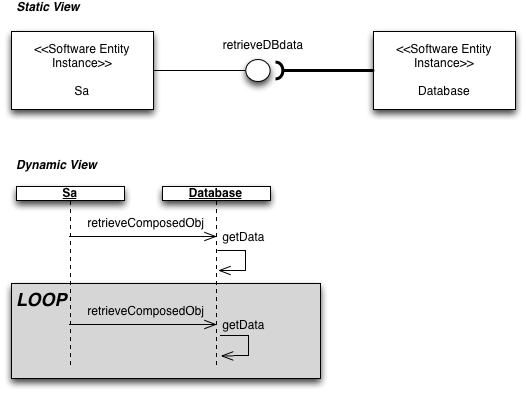
\includegraphics[width=1\textwidth]{./images/circuit.png}
\caption{Circuitous
Treasure Hunt sample \cite{Vetoio2011}}
\label{fig:circuit}
\end{minipage}
\begin{minipage}{.5\textwidth}
\centering
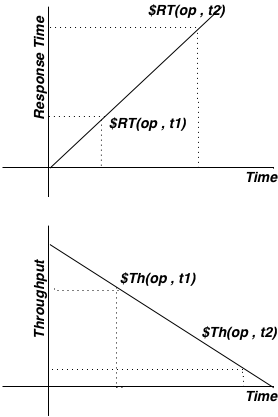
\includegraphics[width=0.5\textwidth]{./images/ramp.png}
\caption{The Ramp sample \cite{Vetoio2011}.}
\label{fig:ramp}
\end{minipage}
\end{figure}



All tests in the experiment were conducted without the need of a tester, automating the process of executing and designing performance test scenarios. This experiment applied four scenarios: Two scenarios with peformance problems (Ramp and Circuitous Treasure), scenarios with no performance problems (Happy Scenario 1, Happy Scenario 2) and mixed scenarios. 

The Ramp and Circuitous Treasure scenarios implement two performance antipatterns.  Circuitous Treasure Hunt antipattern occurs when software retrieves data from a first componet, uses those results in a second component, retrieves data from the second component, and so on, until the last results are obtained \cite{Smith2002} \cite{Smith2003}. The Ramp it is a antipattern where the processing time increases as the system is used. The Ramp can arise in several different ways. Any situation in which the amount of processing required to satisfy a request increases over time will produce the behavior. With the Ramp antipattern, the memory consumption of the application is growing over time. 




The Fig. \ref{fig:fitnessbygeneration1}  presents the fitness value obtained by each metaheuristic. HybridQ metaheuristic obtained the better fitness values.  



\begin{figure}[h]
\begin{minipage}{.5\textwidth}
\centering
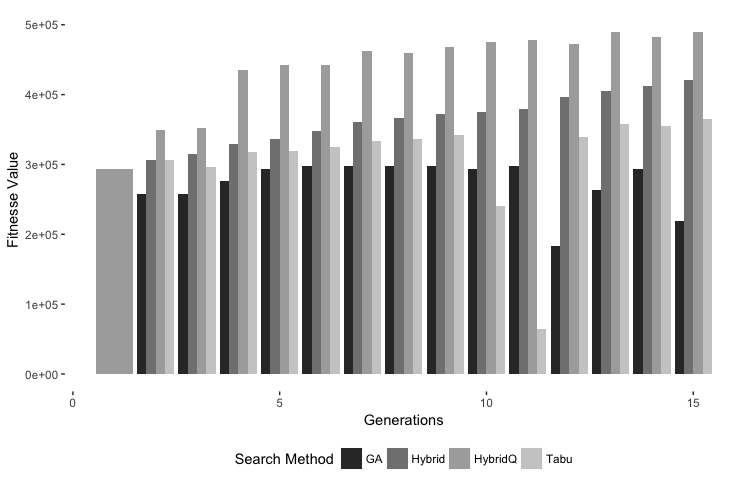
\includegraphics[width=0.7\textwidth]{./images/experiment1-1.png}
\caption{fitness value obtained by Search Method }
\label{fig:fitnessbygeneration1}
\end{minipage}
\begin{minipage}{.5\textwidth}
\centering
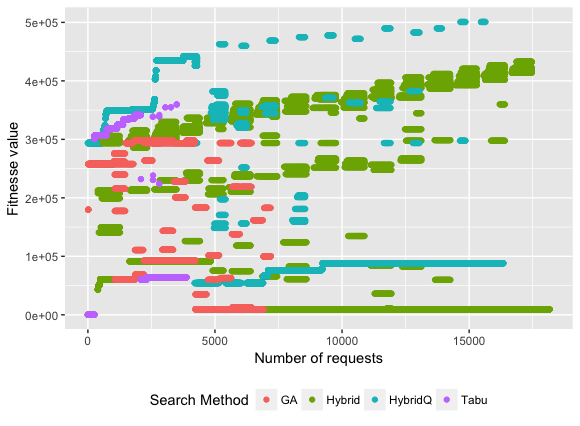
\includegraphics[width=0.8\textwidth]{./images/experiment1-3.png}
\caption{Number of requests by Search Method}
\label{fig:numberofrequestsbysearchmethod}
\end{minipage}
\end{figure}




Despite having obtained the best fitness value in each generation, the Hybrid algorithm performs twice as many requests as the  tabu search (Fig. \ref{fig:numberofrequestsbysearchmethod}). The HybridQ algorithm obtained the best fitness value The Fig. \ref{fig:boxplot1} shows the average, minimal e maximum value by search method.



\begin{figure}[H]
\centering
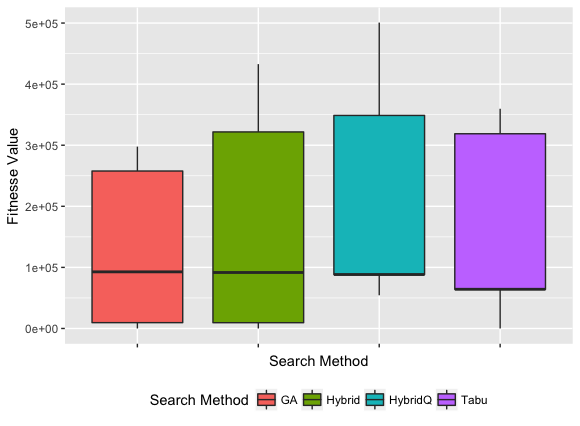
\includegraphics[width=0.8\textwidth]{./images/experiment1-4.png}
\caption{Average, median, maximum and minimal fitness value by Search Method}
\label{fig:boxplot1}

\end{figure}

The Fig. \ref{fig:summaryboxplot1} presents the maximum, average, median and minimum fitness value by generation. The maximun fitness value increases at each generation. The Fig. \ref{fig:density1} presents the density graph of number of users by fitness value. The range between 100 and 150 users has the highest number of individuals found with higher fitness value.

\begin{figure}[H]
\begin{minipage}{.5\textwidth}
\centering
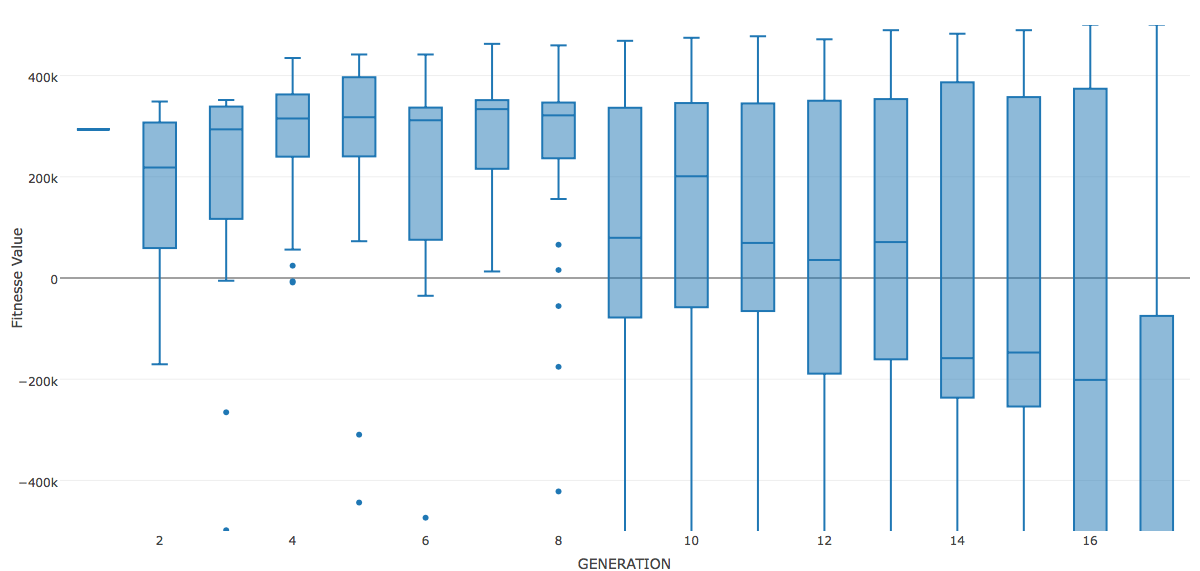
\includegraphics[width=1\textwidth]{./images/experiment1-5.png}
\caption{fitness value by generation}
\label{fig:summaryboxplot1}
\end{minipage}
\begin{minipage}{.5\textwidth}
\centering
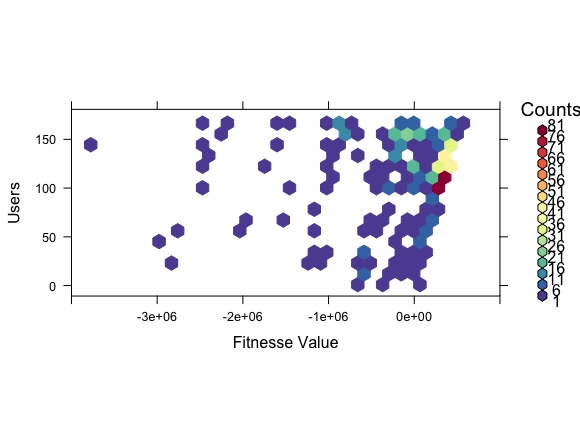
\includegraphics[width=1\textwidth]{./images/experiment1-6.png}
\caption{Density graph of number of users by fitness value}
\label{fig:density1}
\end{minipage}
\end{figure}

Table \ref{tab:bestindividuals} shows 4 individuals with 164 to 169 users. These are the scenarios with the maximum number of users found with the best response time. The first individual has 153 users on Happy Scenario 2, 16 users on Happy Scenario 1 and a response time of 13 seconds. None of the best individuals has one of the antipatterns used in the experiment.



% Please add the following required packages to your document preamble:
% \usepackage[table,xcdraw]{xcolor}
% If you use beamer only pass "xcolor=table" option, i.e. \documentclass[xcolor=table]{beamer}
\begin{table}[h]
\centering
\caption{Best individuals found in the first experiment}
\label{tab:bestindividuals}
\begin{tabular}{lllllll}
\rowcolor[HTML]{C0C0C0} 
\textbf{Search Method} & \textbf{Generation} & \textbf{Users} & \textbf{fitness Value} & \textbf{Happy 2} & \textbf{Happy 1} & \textbf{Resp. Time} \\
HybridQ & 17 & 169 & 500740 & 153 & 16 & 13 \\
HybridQ & 16 & 169 & 500700 & 153 & 16 & 15 \\
HybridQ & 13 & 164 & 489740 & 149 & 15 & 13 \\
HybridQ & 15 & 164 & 489740 & 149 & 15 & 13
\end{tabular}
\end{table}

Fig. \ref{fig:responsetimegenerationalltests1} presents the response time by number of users of individuals with Happy Scenario 1 and Happy Scenario 2. The Figure illustrates that the individuals with best fitness value has more users and minor response time. The Fig. \ref{fig:fitnessgenerationalltests1-1} presents the response time by number of users of individuals with the Ramp and Circuitous Treasure antipatterns scenarios. The Figure illustrates the smallest number of individuals with the antipatterns when compared to individuals who use the happy scenarios.


\begin{figure}[H]
\centering
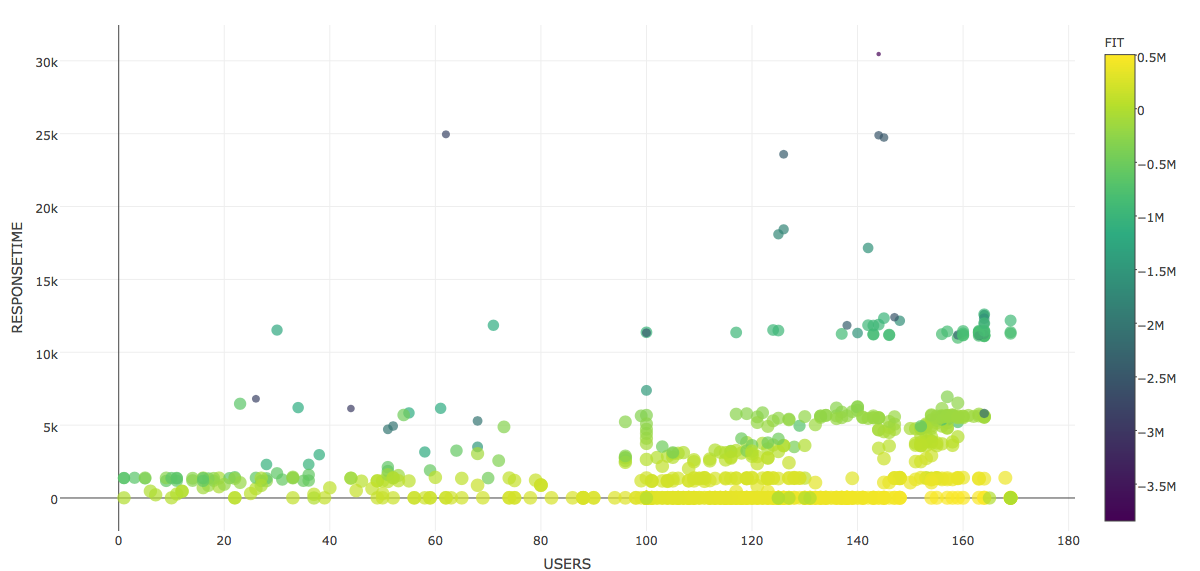
\includegraphics[width=1\textwidth]{./images/experiment1-7.png}
\caption{Response time by number of users of individuals with Happy Scenario 1 and Happy Scenario 2}
\label{fig:responsetimegenerationalltests1}
\end{figure}


Fig. \ref{fig:mdpexperiment1} presents the markov decision process for the experiment. When the response time it is bellow or equal the service level, the action with major reward it is increase the number of users and include more positions with the Happy Scenario 2 (Happy 2). When the response time is above the service level, the action with major reward value it is decrease the number of users and include more positions with the Happy Scenario 2. The actions  with minor value of reward contais the both antipatterns Circuitous Treasure (CTH) and The Ramp antipatterns (Ramp).

In the first experiment, We conclude that the metaheuristics converged to scenarios with an happy path, excluding the scenarios with antipatterns. The hybridQ and hybrid metaheuristic returned individuals with higher fitness scores. However, the Hybrid metaheuristic made twice as many requests than Tabu Search to overcome it. 

\begin{figure}[h]
\begin{minipage}{.5\textwidth}
\centering
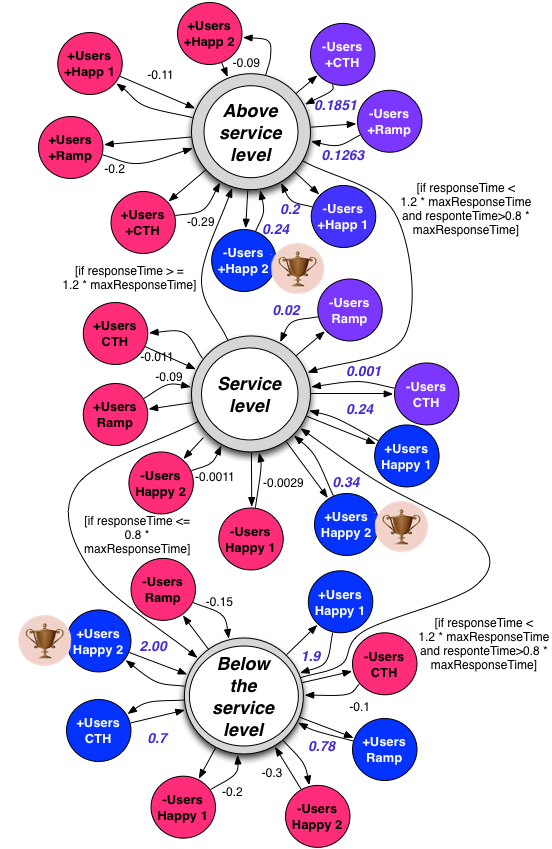
\includegraphics[width=0.7\textwidth]{./images/mdpexperiment.png}
\caption{Markov decision process of experiment with Circuitous Treasure and The Ramp antipatterns}
\label{fig:mdpexperiment1}
\end{minipage}
\begin{minipage}{.5\textwidth}
\centering
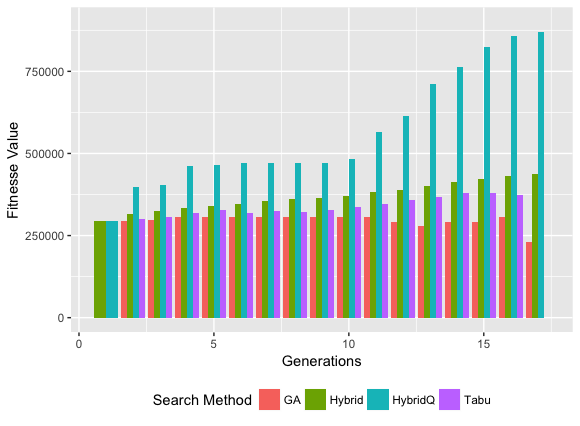
\includegraphics[width=.9\textwidth]{./images/experiment2-7.png}
\caption{Fitness value obtained by Search Method}
\label{fig:fitnessbygeneration2}
\end{minipage}
\end{figure}



\subsection{JPetStore Application Experiments}

One experiment was conducted to test the use of the HybridQ algorithm in a real implemented application. The chosen application was the JPetStore, available at \url{https://hub.docker.com/r/pocking/jpetstore/}. The maximum tolerated response time in the test was 10 seconds.  Any  individuals who obtained a time longer than the stipulated maximum time suffered penalties.  The whole process of stress and performance tests, which took 2 days and about 1800 executions, was carried out without the need for monitoring by a test designer. The tool automatically selected the next scenarios to be run up to the limit of eleven generations previously established. The experiments use the follow application features:


\begin{itemize}
\item Enter in the Catalog: the application presents the catalog of pets.
\item Fishs: The application shows the recorded fishs items.
\item Register:  a new user realize the register in the system.
\item Dogs: The application shows the recorded dogs items.
\item Shopping Cart: the application presents the shopping cart.
\item Add or Remove in Shopping Cart: the application adds and removes items from shopping cart.
\end{itemize}


The experiment used the following fitness function:

\begin{equation}
\begin{aligned}
fitness=\begin{cases} n*\{3000*numberOfUsers-20* 90percentiletime-20*80percentiletime\\-20*70percentiletime
-20*maxResponseTime-penalty\} , \textsf{where n is the }\\\ \textsf{ number of features used by the test in a set of previous selected application} \\ \textsf{features}
\end{cases}
\end{aligned}
\end{equation}


The purpose of the fitness function is to maximize the number of users and minimize the response time in the tests containing the selected functionalities. For example, it is possible double the fitness value for tests that have the fish lookup feature and user registration.


This experiment tries to find the scenarios with maximal number of users and best response time tests that contains the Cart and Register features. The Fig. \ref{fig:experiment31} and \ref{fig:experiment32} show the fitness value by generation. The HybridQ obtained the best fitness values in all generations.

\begin{figure}[h]
\begin{minipage}{.5\textwidth}
\centering
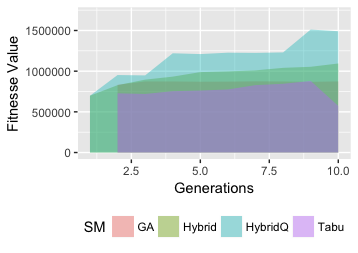
\includegraphics[width=1\textwidth]{./images/experiment3-1.png}
\caption{Fitness value by generation on JPetStore First experiment}
\label{fig:experiment31}
\end{minipage}
\begin{minipage}{.5\textwidth}
\centering
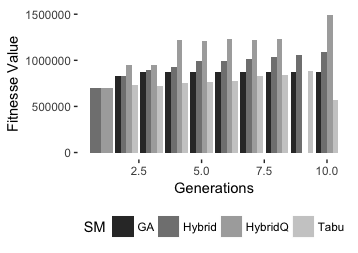
\includegraphics[width=1\textwidth]{./images/experiment3-2.png}
\caption{Fitness value by generation on JPetStore First experiment}
\label{fig:experiment32}
\end{minipage}
\end{figure}

The Fig. \ref{fig:numberofrequestsbysearchmethod3} shows the fitness value by number of request by each Search Method. In the Figure, it is possible to observe that HybridQ obtained the best fitness value to same number of requests of the other algorithms.

\begin{figure}[h]
\begin{minipage}{.5\textwidth}
\centering
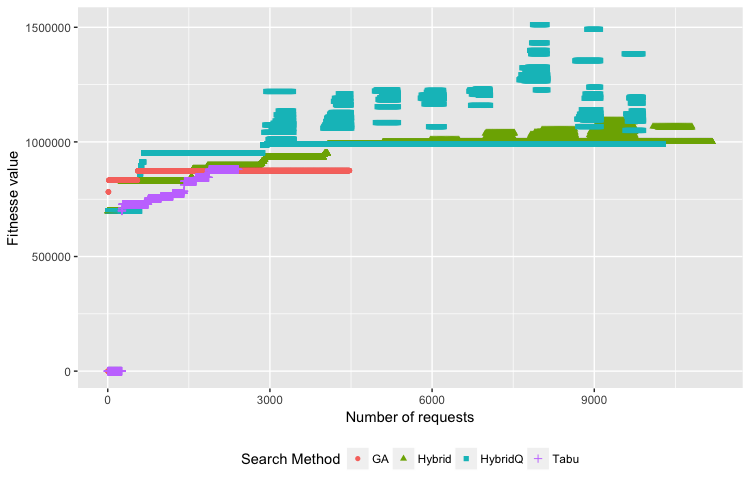
\includegraphics[width=1\textwidth]{./images/experiment3-3.png}
\caption{Number of requests by Search Method}
\label{fig:numberofrequestsbysearchmethod3}
\end{minipage}
\begin{minipage}{.5\textwidth}
\centering
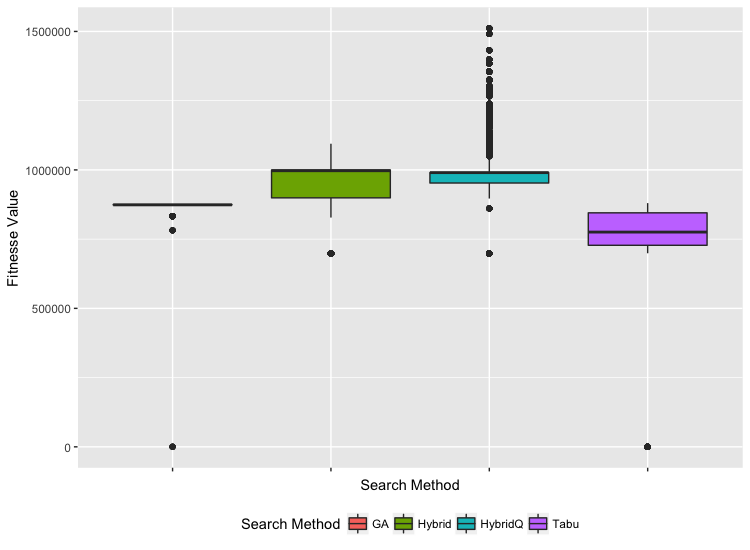
\includegraphics[width=1\textwidth]{./images/experiment3-4.png}
\caption{Fitness value by generation in all tests}
\label{fig:boxplot3}
\end{minipage}

\end{figure}

The Fig. \ref{fig:summaryboxplot3} presents the maximum, average, median and minimum fitness value by generation. The maximun fitness value increases at each generation. Table \ref{tab:bestindividuals3} shows 4 individuals with 233 to 398 users.  The first individual has 73 users on Fishs scenario, 17 users on Dogs scenario, 50 users on Cart scenario, 33 Users on register scenario  and a response time of 357 seconds. 

\begin{figure}[h]
\centering
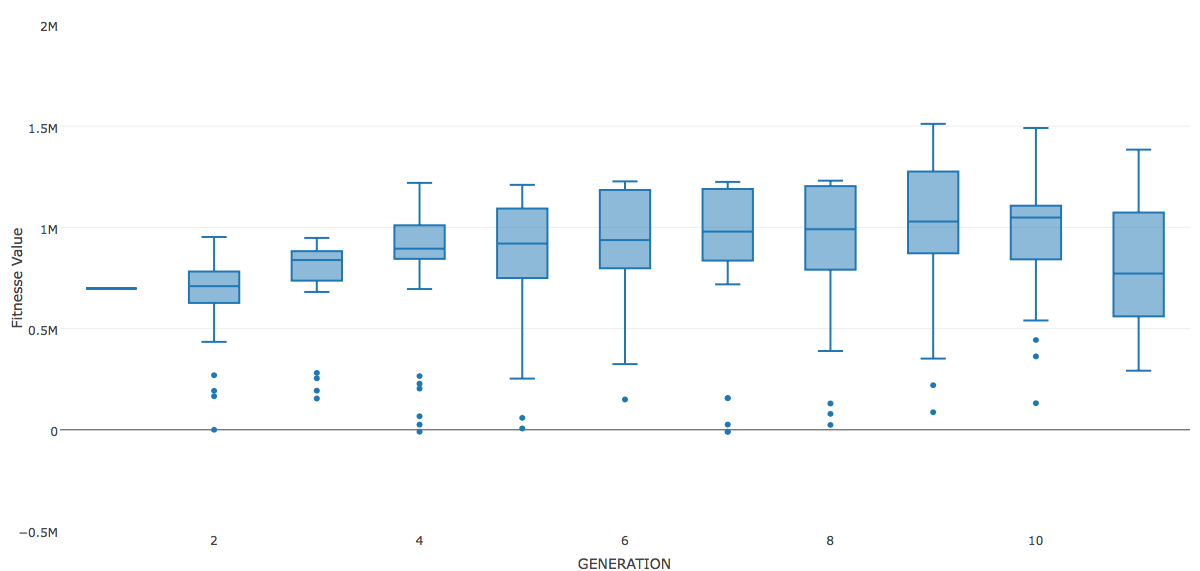
\includegraphics[width=1\textwidth]{./images/experiment3-5.png}
\caption{Average, median and minimum fitness value by Search Method }
\label{fig:summaryboxplot3}
\end{figure}




% Please add the following required packages to your document preamble:
% \usepackage[table,xcdraw]{xcolor}
% If you use beamer only pass "xcolor=table" option, i.e. \documentclass[xcolor=table]{beamer}
\begin{table}[h!]
\centering
\caption{Best individuals found in JPetStore first experiment}
\label{tab:bestindividuals3}
\begin{tabular}{lllllllll}
\rowcolor[HTML]{C0C0C0} 
\textbf{Search Method} & \textbf{Response} & \textbf{Users} & \textbf{Gen} & \textbf{Fitness} & \textbf{Fishs} & \textbf{Dogs} & \textbf{Cart} & \textbf{Register} \\
HybridQ                & 357               & 173            & 9            & 44773            & 73             & 17            & 50            & 33                \\
HybridQ                & 398               & 171            & 10           & 44831            & 57             & 33            & 48            & 33                \\
HybridQ                & 331               & 164            & 9            & 44774            & 71             & 14            & 51            & 28                \\
HybridQ                & 233               & 159            & 9            & 44783            & 63             & 31            & 32            & 33               
\end{tabular}
\end{table}

We conclude that the individuals with major number of uses the four scenarios. The scenario with major number of users is the Fish search feature. The hybrid metaheuristic with Q-Learning (HybridQ) returned individuals with higher fitness scores.  The individual with best fitness value has 73 users on Fishs scenario, 17 users on Dogs scenario, 50 users on Cart scenario, 33 Users on register scenario  and a response time of 357 seconds. 


\section{Conclusion}

IAdapter Testbed is an open-source facility that provides software tools for search based test research. The testbed tool emulates test scenarios in a controled environment using mock objects and implementing performance antipatterns.  Two experiments were conducted to validate the proposed approach. The experiments uses genetic, algorithms, tabu search, simulated annealing and an hybrid approach proposed by Gois et al. \cite{Gois2016}.

The experiments ran for 17 generations. The experiments used an initial population of 4 individuals by metaheuristic. All tests in the experiment were conducted without the need of a tester, automating the execution of stress tests with the JMeter tool.

In both experiments the hybrid metaheuristic returned individuals with higher fitness scores. However, the Hybrid metaheuristic made twice as many requests than Tabu Search to overcome it. The SA algorithm obtained the worst fitness values. The algorithm initially used a scenario with an antipattern and found neighbors that still using the antipatterns over the 17 generations of the experiment.

In the first experiment the metaheuristics converged to scenarios with an happy path, excluding the scenarios with the use of an antipatterns. The individual with best fitness value has 64 users on Happy Scenario 2, 81 users on Happy Scenario 1 and a response time of 12 seconds. None of the best individuals has one of the antipatterns used in the experiment.


In the second experiment,  the metaheuristics converged to scenarios with an happy path and Tower Babel antipattern, excluding the scenarios with Unbalanced Processing antipattern. The individual with best fitness value has 72 users on Happy Scenario 2, 30 users on Happy Scenario 1, 46 user with the antipattern Tower Babel and a response time of 11 seconds. Future works include the use of new antipatterns and more experiments with the use of the antipattern Tower Babel.





%\begin{acknowledgements}
%If you'd like to thank anyone, place your comments here
%and remove the percent signs.
%\end{acknowledgements}

% BibTeX users please use one of
%\bibliographystyle{spbasic}      % basic style, author-year citations
%\bibliographystyle{spmpsci}      % mathematics and physical sciences
%\bibliographystyle{spphys}       % APS-like style for physics
%\bibliography{}   % name your BibTeX data base

\bibliographystyle{spphys}
\bibliography{bibfile}

% Non-BibTeX users please use
%\begin{thebibliography}{}
%
% and use \bibitem to create references. Consult the Instructions
% for authors for reference list style.
%
%\bibitem{RefJ}
% Format for Journal Reference
%Author, Article title, Journal, Volume, page numbers (year)
% Format for books
%\bibitem{RefB}
%Author, Book title, page numbers. Publisher, place (year)
% etc
%\end{thebibliography}

\end{document}
% end of file template.tex

